The conference begins! Today we have a few keynotes and the workshops.


\subsection{Keynote: Cynthia Dwork on Recent Developments in Algorithmic Fairness}

The field (of algorithmic fairness) began around 2010, but today we'll talk about brand new developments.

\subsubsection{Algorithmic Fairness}

{\bf Point 1:} Algorithms are unfair, data are unrepresentative, labels can embody bias. \\

{\bf Point 2:} Algorithms can have {\it life altering consequences}.
\begin{itemize}
    \item Mortgage terms.
    \item Detention/release.
    \item Medical assessments and care.
    \item Deciding if a child is removed or not from a home.
\end{itemize}

$\ra$ Lots of papers that say: ``we're shocked by these examples of algorithmic bias!". But now we're in a position to do something about it. \\

{\bf Algorithmic Fairness:}
\begin{enumerate}
    \item Natural desiderata of fairness conflict with each other
    \item One piece of an unfair world. Deployment can be unfair, too
\end{enumerate}

{\bf Goal:} Develop a {\it theory} of algorithmic fairness. Two groups of fairness definitions:
\begin{enumerate}
    \item Group fairness
    \item Individual fairness
\end{enumerate}

\ddef{Group Fairness}{Statistical requirements about the relative treatment of two disjoint groups.}

Example of group fairness: demographics of students accepted to a college should be equal. Or, balance for positive/negative class.\\


\ddef{Individual Fairness}{People who are similar with respect to a given classification task should be treated similarly}

$\ra$ Comes from a strong legal foundation.\\


Problems:
\begin{itemize}
    \item Group notions fail under scrutiny
    \item Individual fairness requires a task specific metric.
    
    $\ra$ Paucity of work on individual fairness because we need such specific metrics.
\end{itemize}


\subsubsection{Approaches to Fairness}

Metric Learning for Algorithmic Fairness:
\begin{itemize}
    \item Adjudicator has an intuitive mapping from high dimensional feature vector ($X$) to the important aspects of the problem ($Z$).
    \item Relative queries are easy (which of $A$ and $B$ is closer to $C$?)
    \item Absolute queries are hard (what is $d(A,B)$?)
    $\ra$ Idea: turn to learning theory.
    \item Three insights in trying to answer above adsolute queries:
    \begin{enumerate}
        \item Distance from a single representative element produce useful approximations to the true metric.
        \item Parallax can be achieved by aggregating approximations obtained from a small number of representatives.
        \item Can generalize to unseen elements.
    \end{enumerate}
    \item See also: Bridging the Group vs Individual Gap~\cite{hebert2018multicalibration,kim2018fairness}:
\end{itemize}


\subsubsection{Hybrid Group/Individual Fairness Approaches}

Consider individual probabilities: 1) what is the probability that $P$ will repay a loan? 2) What is the probability that a tumor will metastasize?, and so on. \\

$\ra$ One concern: these events will just happen once. How should we think about these in terms of giving medical/legal recommendations? How can we justify the answer? \\

Philip Dawid wrote a recent survey of individual fairness definitions~\cite{dawid2017individual}. \\

One idea: calibration. Consider forecasting the weather. When we say $30\%$ chance of rain, we mean that $30\%$ of the days we predict $30\%$ rain will rain, and $70\%$ will not. \\

{\bf The Tumor Example:} Expectations are obtained from binary outcome data.

$\ra$ Study A says 40\% chance of a tumor, and Study B says $70\%$ (but not training data/context, just the studies output). \\

So, given $C = \{S_1, S_2\}$, consider the venn diagram formed by the recommendation of the two studies. We can choose values for elements $P = S_1 \ S_2$, $Q = S_1 \cap S_2$, and $R = S_2 \ S_1$, that retain the given expectations. This can help us clarify the appropriate decision. \\

But: many multi-accurate solutions. If, however, we had ensured calibration, we {\it can} narrow down the expectation to something accurate. \\

{\bf The Loan Example:}
\begin{itemize}
    \item Intersecting demographic/ethnic/age/gender/etc/ groups.
    \item Minimally: policies consistent with expected repayment rates for each group.
\end{itemize}

Q: Who decides which groups should be prioritized? The culturally dominant? The oppressed? How do we set our scoring function? Really hard question~\cite{jost1994role} \\

A: Let's turn to complexity theory! \\
$\ra$ All grouds identifiable by small circuits acting on the given data.

\begin{conjecture}
Captures all historically disadvantaged groups $S$.
\end{conjecture}

Multi-accuracy and multi-calibration: we can do it!
\begin{itemize}
    \item Multi-Accuracy: Complexity of creating the scoring function depends on hardness of (agnostic) learning of $C$, but function is efficient.
    \item Multi-calibration: $f$ is calibrated on each set $S \in C$ simultaneously, accurate in expectation.
\end{itemize}

{\bf Problem:} The Devil is in the collection of $C$. \\

$\ra$ We hope we capture task specific semantically significant differences. \\

Q: What are the sources of information available to child protective services and call screening?

\subsubsection{Fair Ranking}

Q: Why? \\

A1: Ranking is crucial to many endeavors: the heart of triage, underlying impetus for scoring, rank translates to policies or to scores in clinical trials.\\

A2: Thinking about ranking can help us in thinking about a scoring function more generally. \\

{\bf Idea:} Let's think about fair ranking from the cryptographic perspective. \\

Rank Unfairness:
\begin{itemize}
    \item Suppose we have two groups of people: $A$ and $B$.
    \item Suppose $\bE[A] > \bE[B]$.
    \item But! It's silly to then rank everyone in $A$ above everyone in $B$.
\end{itemize}

Take a cryptographic/complexity theoretic approach to address this problem!

$\ra$ If positive and negative examples are computationally indistinguishable, the best one can do is assign to everyone a probability according to the base rate.

\subsubsection{Approaches from Representation Learning}

{\bf Idea:} Learn a ``fair" representation (in group fairness).
\begin{itemize}
    \item Stamps out sensitive information (``censoring")
    \item Retains sufficient information to permit standard training.
\end{itemize}

Goal: learn a censored mapping to a lower dimensional space $Z$~\cite{edwards2015censoring}.
\begin{itemize}
    \item Encoder tries to hide memership bit, permit prediction on $Z$.
    \item Decoder tries to reconstruct $x$ from $z = Enc(x)$
    \item Adversary $(A)$ tries to distinguish $Enc(x \in S)$ from $Enc(x \in S^c)$.
\end{itemize}

$\ra$ Approach by~\citet{madras2018learning} tie this objective to scoring, show that transfer is possible. \\

\begin{figure}[h!]
    \centering
    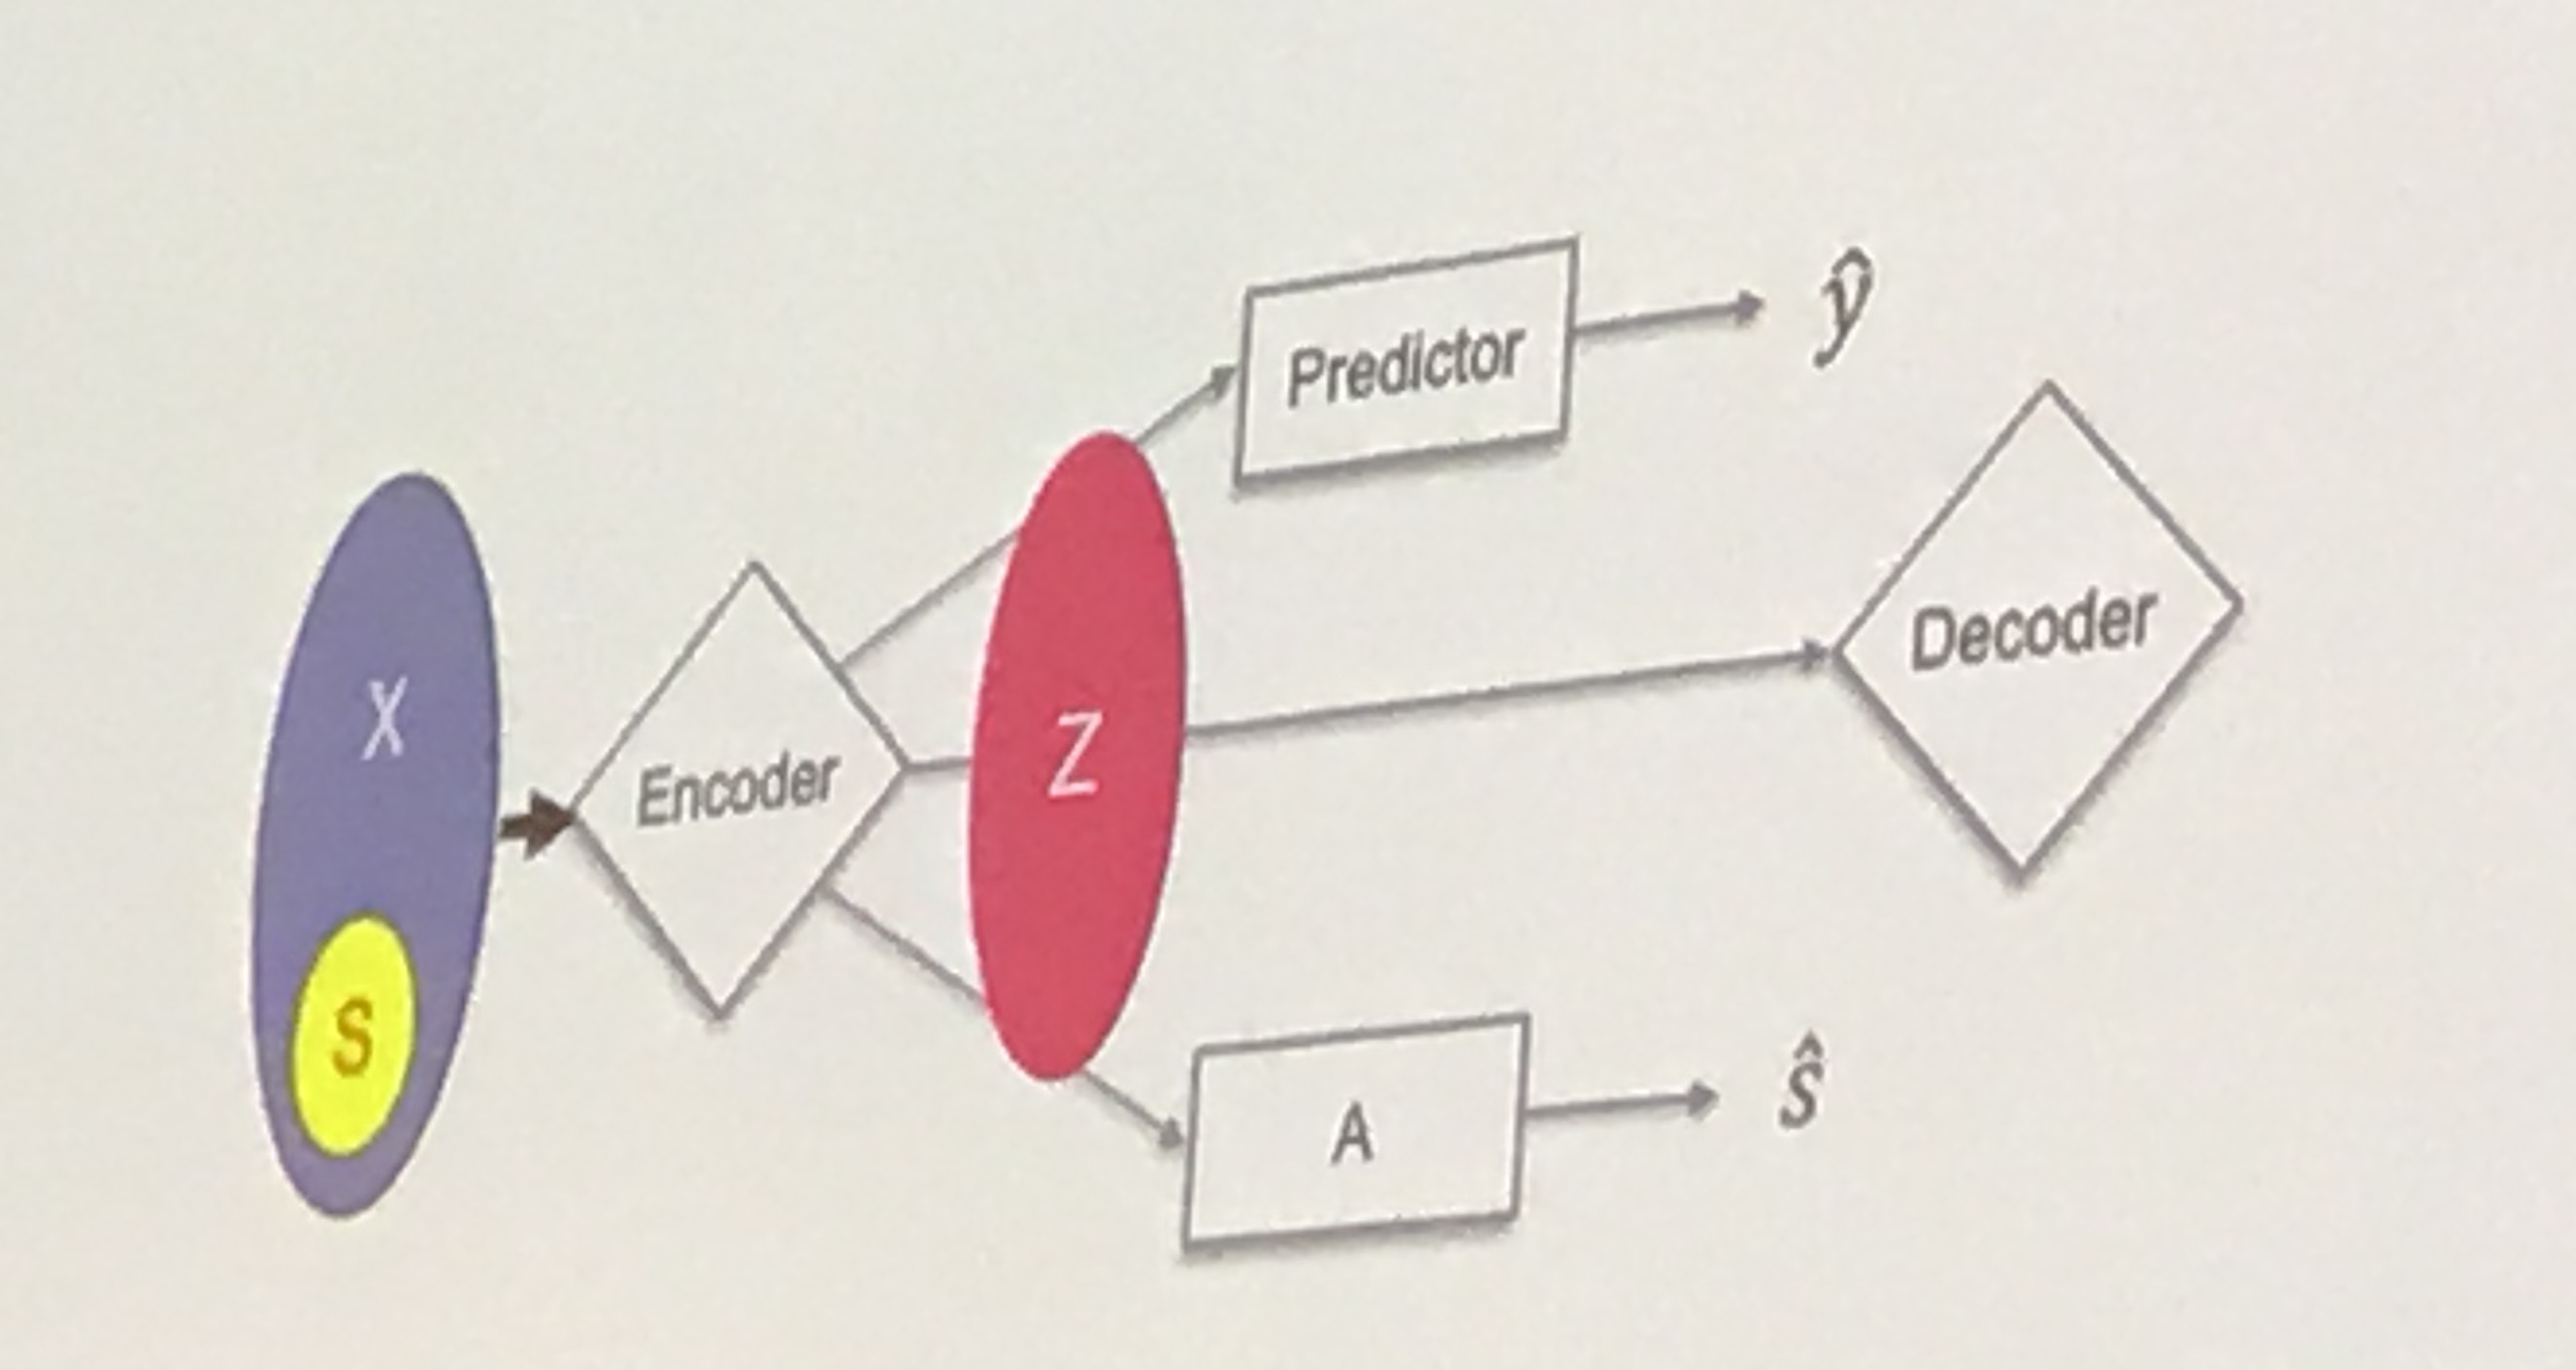
\includegraphics[width=0.4\textwidth]{images/code_rep.png}
    \caption{The cryptographic setup for learning fair representations.}
    \label{fig:my_label}
\end{figure}

{\bf The Harvard-Stanford Problem:} Suppose you're at Stanford, and you build an algorithm for detecting tumors that works really well. Suppose someone else is at Harvard and does the same. \\

$\ra$ Claim: the algorithms wont work across the populations due to differences in the groups and in the lab settings. \\

Goal, then, is to find a way to identify differences/similarities across populations so that these methods {\it can} be transferred across populations.

Approach:
\begin{itemize}
    \item Choose $y \sim Bernoulli(\text{base rate})$
    \item Choose $x \sim N(\mu, \Sigma)$
    \item Retain $x$ if $Bernoulli(\sigma(f_1,s_1)) = f_26i(x_2) = y$.
\end{itemize}


Summary:
\begin{itemize}
    \item A fair algorithm is only one piece of an unfair world
    \item Multiple kinds of fairness: group, individual, Multi-X.
    \item Breakthrough in metric learning for individual fairness
    \item Individual probabilities are hard to understand, but we can  learn from fairness methods to improve their use.
    \item Censered representations and out-of-distribution generalization.
\end{itemize}

\spacerule


Now off to the Structure and Priors in Reinforcement Learning workshop!


\subsection{SPiRL Workshop}
\label{sec:spirl}

First, Pieter Abbeel on Model-based RL!

\subsubsection{Pieter Abbeel on Model-Based RL from Meta RL}

Few-shot RL/Learning to RL: we have a {\it family} of environments, $M_1, M_2, \ldots, M_n$. Hope is that when we learn from these $n$ environments, we can learn faster on environment $M_{n+1}$. \\

Fast Learning:
\begin{equation}
    \max_\theta \bE_M \bE_{\tau_M} \left[\nsum R_\tau_M^i \mid \text{RLAgent}_\theta \right].
\end{equation}

Objective is roughly the above, where we ground \text{RLAgent}$_\theta$ as an RNN (or some othe generic computational architecture). \\

Other ways to solve this objective like Model-Agnostic Meta Learning (MAML)~\cite{finn2017model}. \\

{\bf Point:} Family of methods that let you train quickly in new environments (new $R$, $T$), given interactions with prior environments. \\

Motivation for Simulation:
\begin{itemize}
    \item Less expensive (can't break robot)
    \item Faster/more scalable
    \item Easier to get lots of labels
\end{itemize}

Q: How can we leverage {\it crude} simulation through domain randomization?  \\

$\ra$ Think about minecraft -- there's some visual structure that is useful for learning about the world, but it's not perfect. How can we train in minecraft (or similar domains) and transfer to the world? \\

A: Randomize aspects of simulations in order to make training of vision system easier. Can then transfer these trained perceptual classifiers to the world, and it works! (same goes for grasping) \\

A: Same goes for grasping -- can train to grasp in simulation, then grasp real objects (with around 80\% success rate). \\

{\bf Result:} Train a hand controller (for manipulating a block in hand) in simulation, can actually deploy it on a real robot. \\

\ddef{Model-Free RL}{Interact with the world and collect data $D$. Then, use this data to inform $\pi$ or $Q$, and use those to act.}

\ddef{Model-Based RL}{Interact with the world and collect data $D$. Then, use this data to inform a world simulator, $\widehat{M}$, perform simulations in order to act.}

Canonical model-based RL;
\begin{enumerate}
    \item For iter $ = 1, 2, \ldots$
    \item \hspace{6mm} Collect data under current policy
    \item \hspace{6mm} Improve learned simulator from all past data
    \item \hspace{6mm} Use simulator to act and collect new data.
\end{enumerate}

{\bf Problem:} learned models are imperfect!  \\

{\bf Fix:} Learn a better simulator. But, this is insufficient. Extremely hard to learn the {\it right} simulation. \\

$\ra$ New overfitting challenge in model-based RL. Policy optimization tends to exploit regularities in simulator, leading to catastrophic failures. \\

{\bf Key Idea:} Don't need to learn an accurate model, just need to learn a set of models representative of the real world (and do few-shot RL):
\begin{enumerate}
    \item For iter $ = 1, 2, \ldots$
    \item \hspace{6mm} Collect data under current adaptive policies, $\pi_1, \ldots, \pi_k$
    \item \hspace{6mm} learn ENSEMBLE of $k$ simulators from past data.
    \item \hspace{6mm} meta-policy optimization over ensemble
    \item \hspace{12mm} new meta-policy $\pi_\theta$
    \item \hspace{12mm} new adaptive policies $\pi_1, \ldots, \pi_k$.
\end{enumerate}

Experiments: 
\begin{enumerate}
    \item {\it MuJoCo:} With about 45 minutes of real interaction with the mujoco environment, state-of-the-art model-free methods can't learn, while the meta-learning approach can.
    \item {\it Robots:} Similarly, can train meta model-based RL in a sample efficient way to learn to perform robotic grasping tasks.
    
    $\ra$ Between 10-100$\times$ more efficient than model-free methods {\it to get to the same asymptotic performance.}
\end{enumerate}

\begin{figure}[h!]
    \centering
    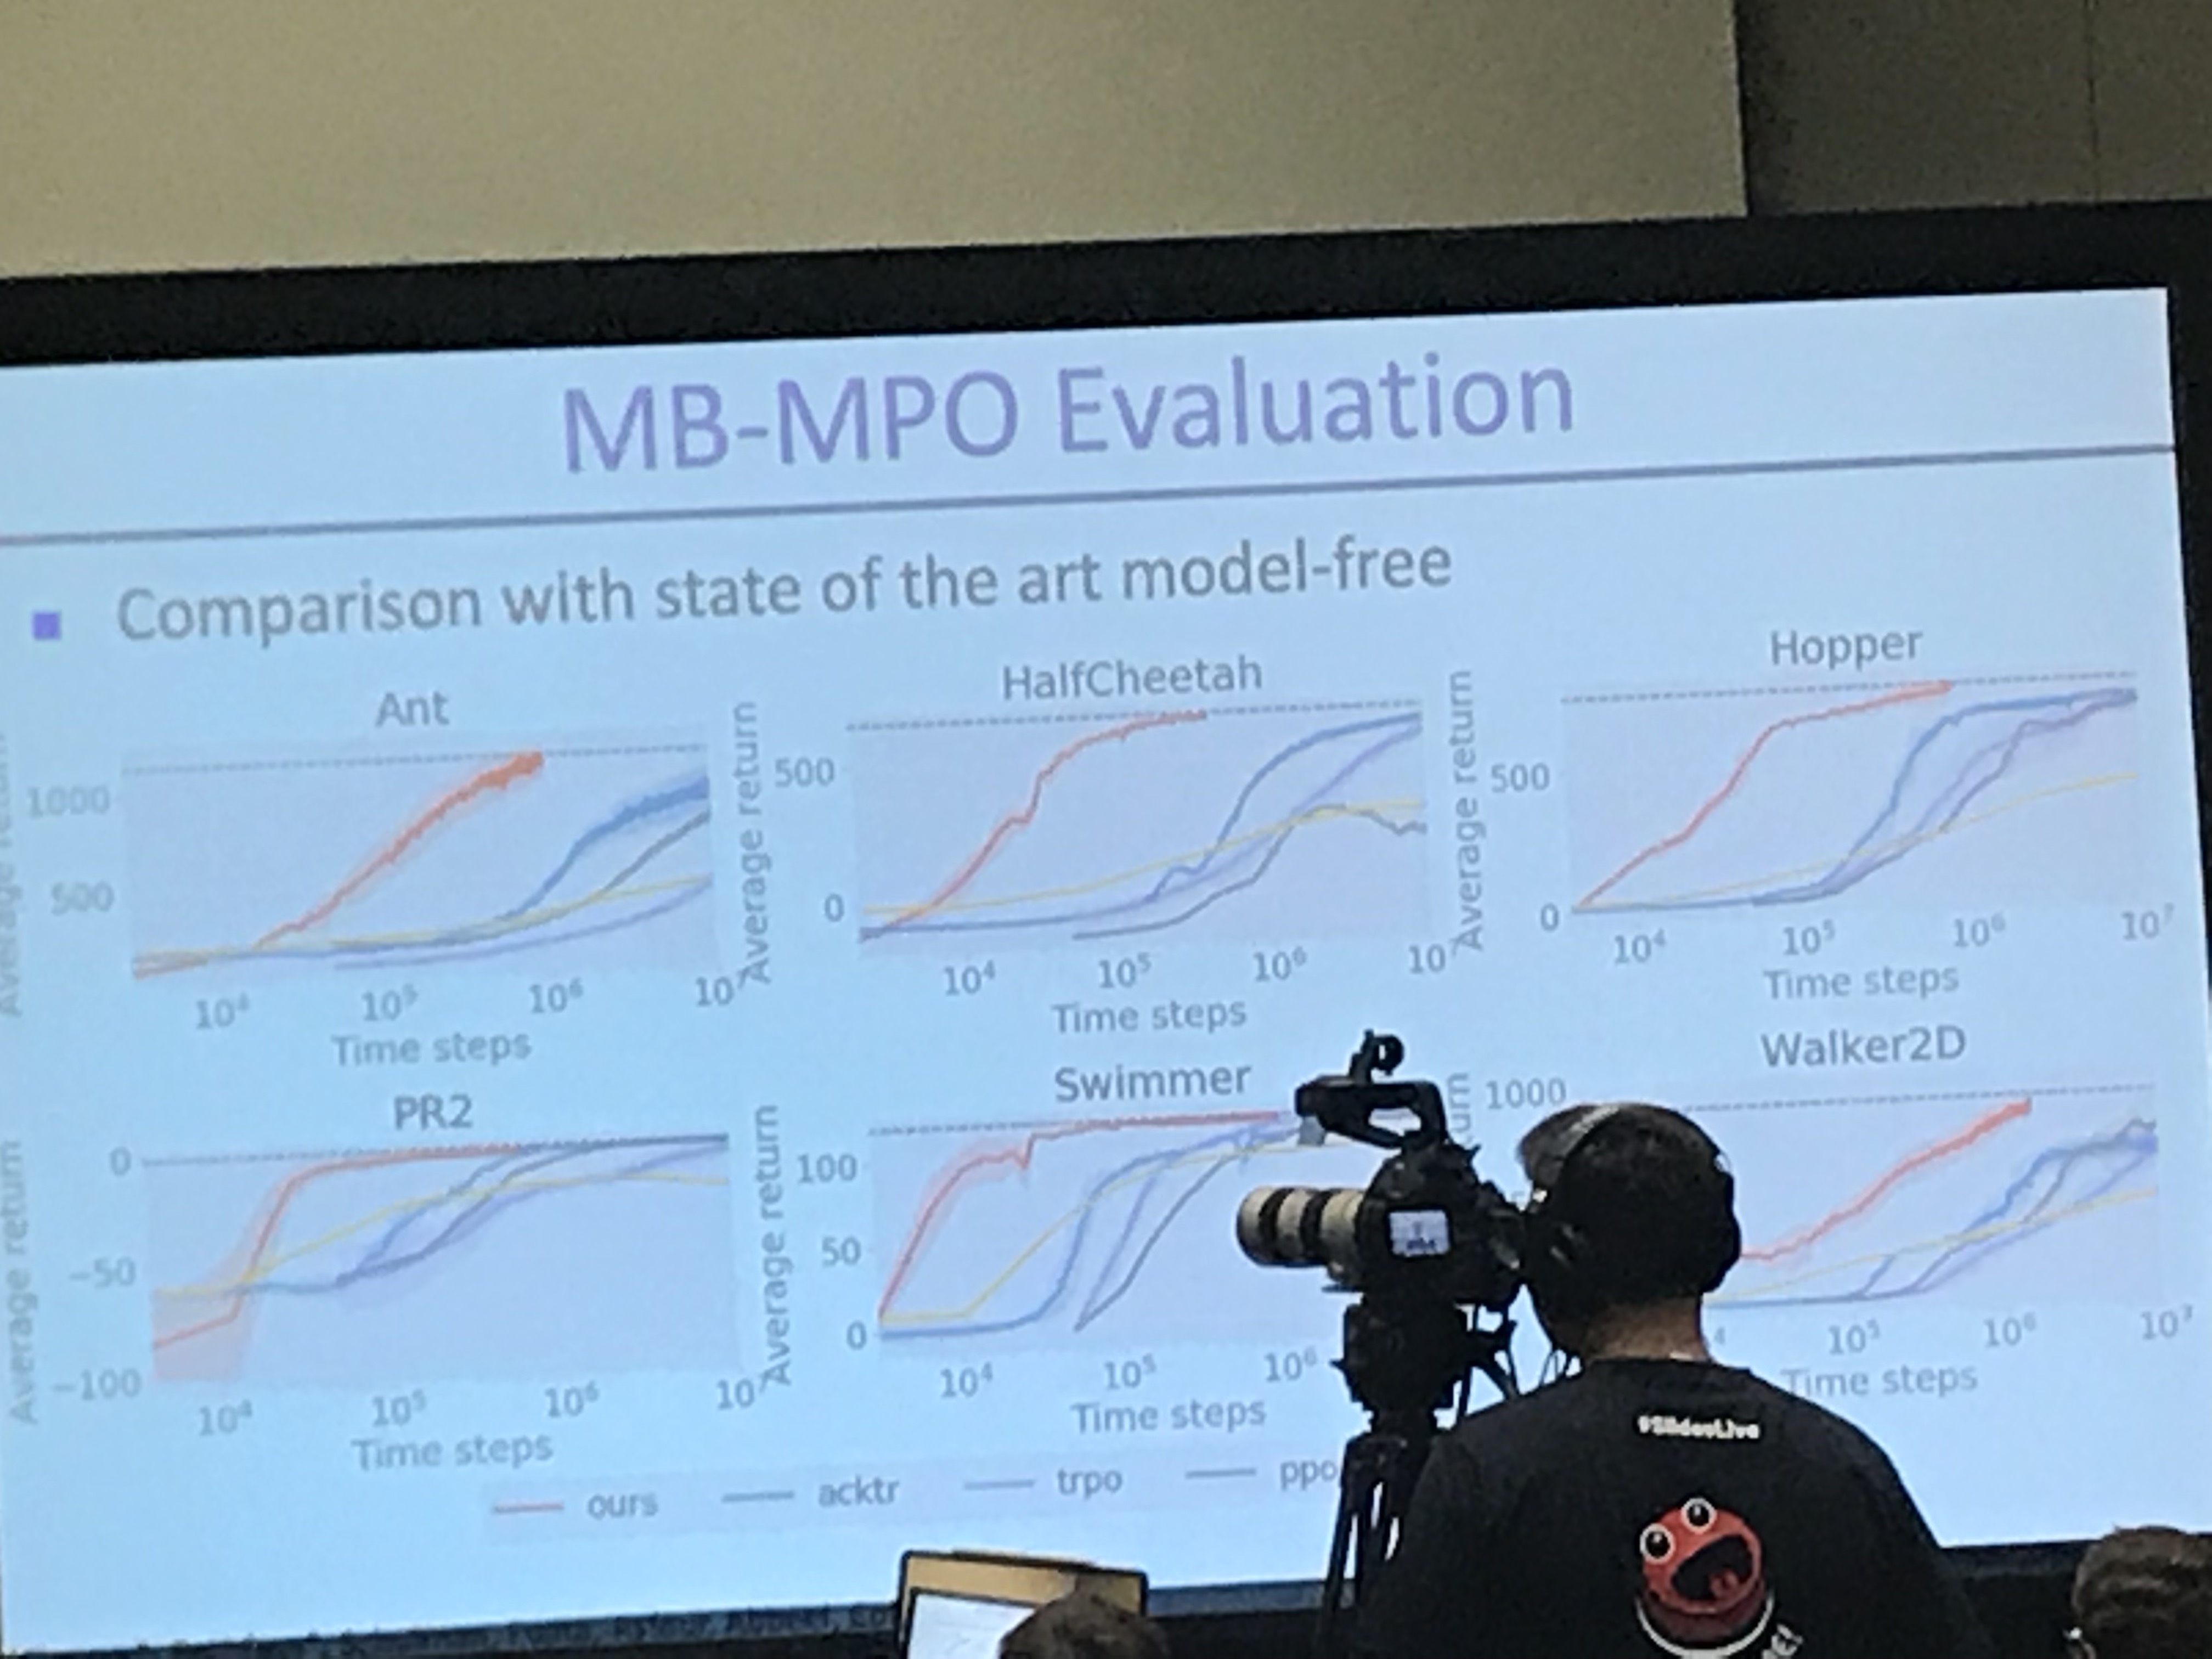
\includegraphics[width=0.4\textwidth]{images/mbrl_results.JPG}
    \caption{Results from meta model-based RL (and a camera + person).}
    \label{fig:meta_mbrl}
\end{figure}


{\it Challenge Question:} Hierarchical RL promises to solve long horizon planning problems. \\

Q1: Are model-free and model-based HRL fundamentally different approaches or are they the same? \\

Q2: Do you think there's a way to combine these two? \\

Pieter A: Yeah absolutely! The methods we presented do some work to combine these methods together. For HRL it might be a bit different, though. In some sense, at the high level, humans don't do RL. We don't have enough ``high level" trials to explore things like ``go to conference/do a PhD". So, the higher level is probably model-based and more planning based rather than RL. Another thing that comes to mind is that HRL approaches seem to only have two levels. One interesting direction is to generalize with more depth/levels rather than two levels. Still not obvious where the separation between model-based/model-free methods takes place. \\

Q: Pros and Cons of looking for an end-to-end approach as opposed to a more modular approach (with more intermittent structure like state estimation). \\

Pieter A: There's no final answer here -- state estimation sometimes involves human provided information, might lose the wrong data for doing control (what is state for a self driving car, for instance?). But, some priors in this way can probably help!


\subsubsection{Contributed Talk: Kate Rakelly on Off Policy RL via Context Variables}

{\bf Goal:} Design agents that are skilled a variety of different tasks. \\

$\ra$ But, training agents in new tasks is statistically/computational infeasible, so really we'd like to exploit shared structure across tasks. \\

{\bf Approach (High-Level):} Meta-RL to learn shared structure across related tasks. \\

Problems: Rapid adaptaion requires efficient exploration strategies, while meta-training requires data from each task, exarcerbates sample inefficiency. \\

{\bf Approach (Detailed View):} Meta-RL via an {\it off-policy} approach. But, raises a problem with exploration since we no longer control the experience distribution. \\

``Context": task-specific information learned from a task ($z$). Meta-training then has two pieces:
\begin{enumerate}
    \item Learn to summarize the context into $z$.
    \item Learn to take actions given $s,z$.
\end{enumerate}

{\bf Algorithm:} \textsc{Pearl}. Given a new task, main idea is to maintain a probability distribution over which task we're in. This lets us exploit knowledge of uncertainty to adapt efficiently to the new task. \\

{\bf Experiments;} four different mujoco domains (half cheetah, humanoid, ant, walker). Rewards and dynamics change across tasks (locomotion direction, velocity, joint parameters). 

Summary:
\begin{itemize}
    \item \textsc{Pearl} is the first off-policy Meta-RL algorithm
    \item 20-100$\timex$ improved sample efficiency on the domains tested
    \item Posterior sampling for efficient exploration during adaption.
\end{itemize}

Code: \url{github.com/katerakelly/oyster} \\

Posters now for a bit.





\subsubsection{Matt Bottvinick on Meta-RL: An Appreciation}

{\bf Point:} We need some structure to scale RL. What I have in mind is something like relational RL, objects, graph nets, and so on. \\

Guiding Question: What do the algorithms that meta-RL gives rise to, do? What can't they do? \\

Recent survey summarizing some of the ideas~\citet{botvinick2019reinforcement}. \\

$\ra$ The field seems to have moved on from meta-RL, but I can't! Let's really understand these algorithms. \\

Tendency: let's build a faster race car. This talk: let's understand fast race cars, or why these things we've made recently are fast! \\

Observations in trying to understand Meta-RL:
\begin{itemize}
    \item Consider two-armed bandits: An animal chooses between two arms, payoff determined according to some payoff schedule. Critically, sources of reward get restocked every so often. 
    
    $\ra$ Animals match their frequency in choices with the frequency with which they get rewards (probability matching).
    
    $\ra$ Ordinary LSTM figures that out, too! Also figures out the gittins optimal thing in the regular $\beta-Bernoulli$ bandit.
    
    \item Consider this new bandit task: probabilities of payoff keep changing, but volatility changes, too (long intervals where payoffs flip around, etc.).
    
    $\ra$ Smart thing is to change your learning rate. People do in fact do this (if we fit a model predicting learning rates to peoples' decisions).
    
    $\ra$ Meta-learned LSTM can do the same thing!
    
    \item Monkey sees two colored face down cups, one of which hides a raisin. Learn to pickup the cup hiding the raisin in general.
    
    $\ra$ Then the monkey has to transfer to a new task with new objects. Turns out monkey learns to transfer as well; when no info can be used, monkey explores uniformly, when info can be exploited, monkey learns very quickly.
    
    $\ra$ LSTM can do this, too!
\end{itemize}

Clear illustration of a meta model-free algorithm giving rise to a model-based RL, based on model-based tests designed for people/animals from~\citet{daw2014algorithmic}. \\

\begin{figure}[h!]
    \centering
    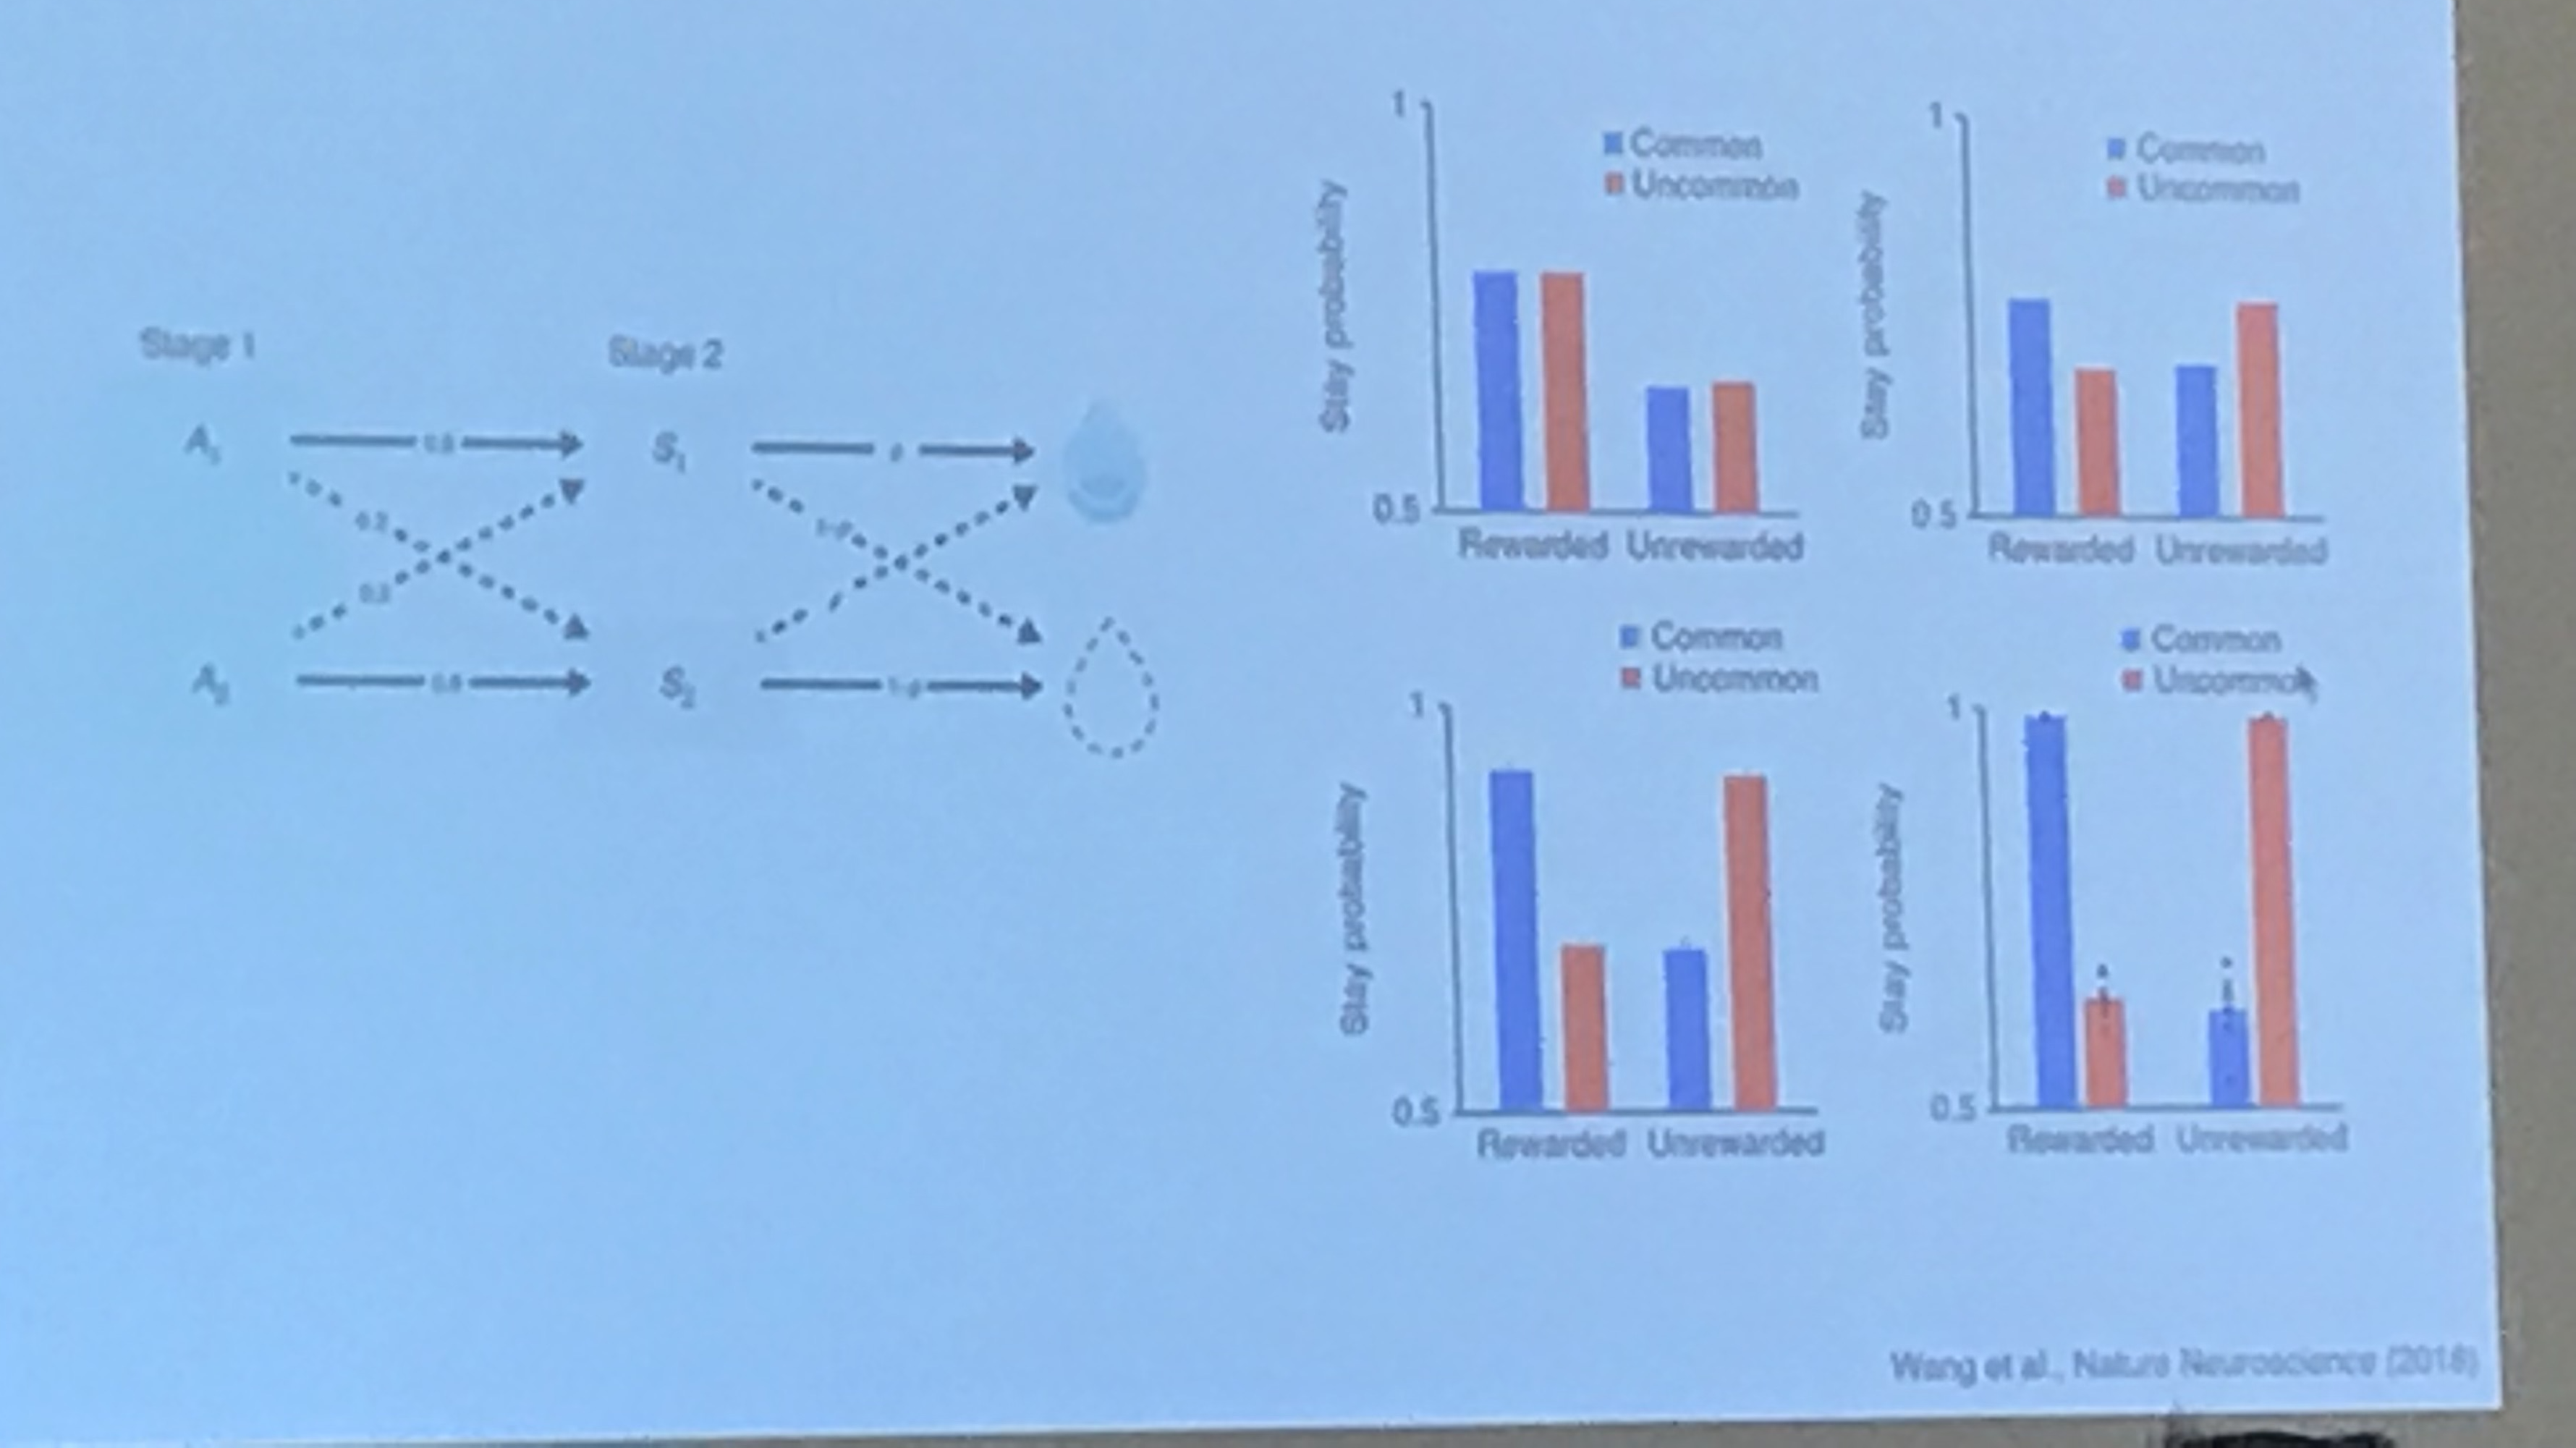
\includegraphics[width=0.4\textwidth]{images/mb_task.png}
    \caption{A task for determining whether a decision making is using model-based techniques or not (left) and results from different approaches on the task (right).}
    \label{fig:mb_task}
\end{figure}

{\bf Point 1:} Meta-RL can also give rise to algorithms that can solve temporal credit assignment problems, too. \\

{\bf Point 2:} For LSTM to be solving certain kinds of tasks, they also must be retaining some sufficient statistics in their state (that roughly match what the observer would track, too). \\

Lastly: a crazy idea (\dnote{Matt's words, not mine :)}). We have some evidence that with ordinary LSTMs, model-free RL can give rise to model-based RL (in the right situation). \\

$\ra$ Maybe, if we set of the environments in the right way, maybe LSTMs can work out algorithms for doing (amortized?) Bayesian inference. \\

{\bf Take Home Message:} Meta-RL is really exciting, let's keep coming up with faster algorithms but also try to understand what they're doing.

\subsubsection{Katja Hoffman on Challenges \& Directions in Multi-Task RL}

Q: Why do we focus on structure and priors in RL? \\

Katja A: Three things!
\begin{enumerate}
    \item Improve sample efficiency
    \item Improve sample efficiency
    \item Improve sample efficiency
\end{enumerate}

Q: When you think about structure and priors in RL, what kidns of challenges become solvable? \\

A: Maybe in games, science, transporation, medicine? \\

$\ra$ For these (and probably other) domains, structure is crucial. \\

%Q: Who will have access to these solutions? \\

Kinds of Structure:
\begin{itemize}
    \item Assume multiple related tasks and useful relationship between tasks can be learned from data
    \item Q: What types of models allow learning and use of related task structure>?
    \item Q: What trade-offs can we achieve between prior assumptions, flexibility, and sample efficiency?
\end{itemize}

First Approach: Meta-RL with Latent Variable Gaussian Processes~\cite{saemundsson2018meta}. IDea:
\begin{itemize}
    \item Problem: assume $p$ task with related dynamics:
    \begin{equation}
        y_t^p - f(x_i^p, h_p) + \eps,
    \end{equation}
    \item Observe data from training tasks
    \item Goal: accurately predict held out test dynamics with minimal additional data

    \item Approach: Model-Based RL via latent variable Gaussian processes. Place a GP prior on global function.
    
    \item Experiments: 1) toy taks, mult-task prediction. Approach is able to disentangle unseen tasks; 2) multi-task cart pole. System can cary in mass and pendulum length, many held out settings of these parameters.
\end{itemize}

Second Approach: (CAVIA) Fast Context Adaptation via Meta-Learning~\cite{zintgraf2018caml}.
\begin{itemize}
    \item Problem: distribution over training and test task $p_{train}$, $p_{test}$.
    \item During meta-training, sample tasks from $p_{train}$, get train/test data for that task
    \item Learn how to adapt quickly on the task by splitting up network into: 1) task specific context parameters $\phi$, and 2) shared parameters $\theta$.
    \item Experiments: 1) supervised learning task; 2) multi-task half cheetah.
    
    $\ra$ CAVIA learns an itnerestable task embedding, captured in context parameters
    $\ra$ Adapts to test tasks with updates to only context parameters -- sheds new light on meta-learning benchmarks.
    $\ra$ Very flexible
\end{itemize}

Follow up: Variational Task Embeddings for Fast Adaptaion in Deep RL. Learns to trade of exploration and exploitation online, while interacting with the environment. VATE can deduce information about the task before seeing any reward. \\


{\bf Point:} As we push forward in RL to harder domains, there might be certain generic structure that tends to work well across many domains. Can we find this unifying structure? \\

$\ra$ One thing that might be needed is a dataset that might rive rise to such structure. To this end: \\

$\ra$ MineRL: competition (\url{minerl.io/competition}) on sample efficient RL using human priors (upcoming at NeurIPS this year), built on top of MALMO~\cite{johnson2016malmo}. \\

Minecraft is massively complex, so offers a great platform for exploring the use of priors in RL. See Figure~\ref{fig:mc_tree} for a sense of the size of the tech tree.

\begin{figure}[h!]
    \centering
    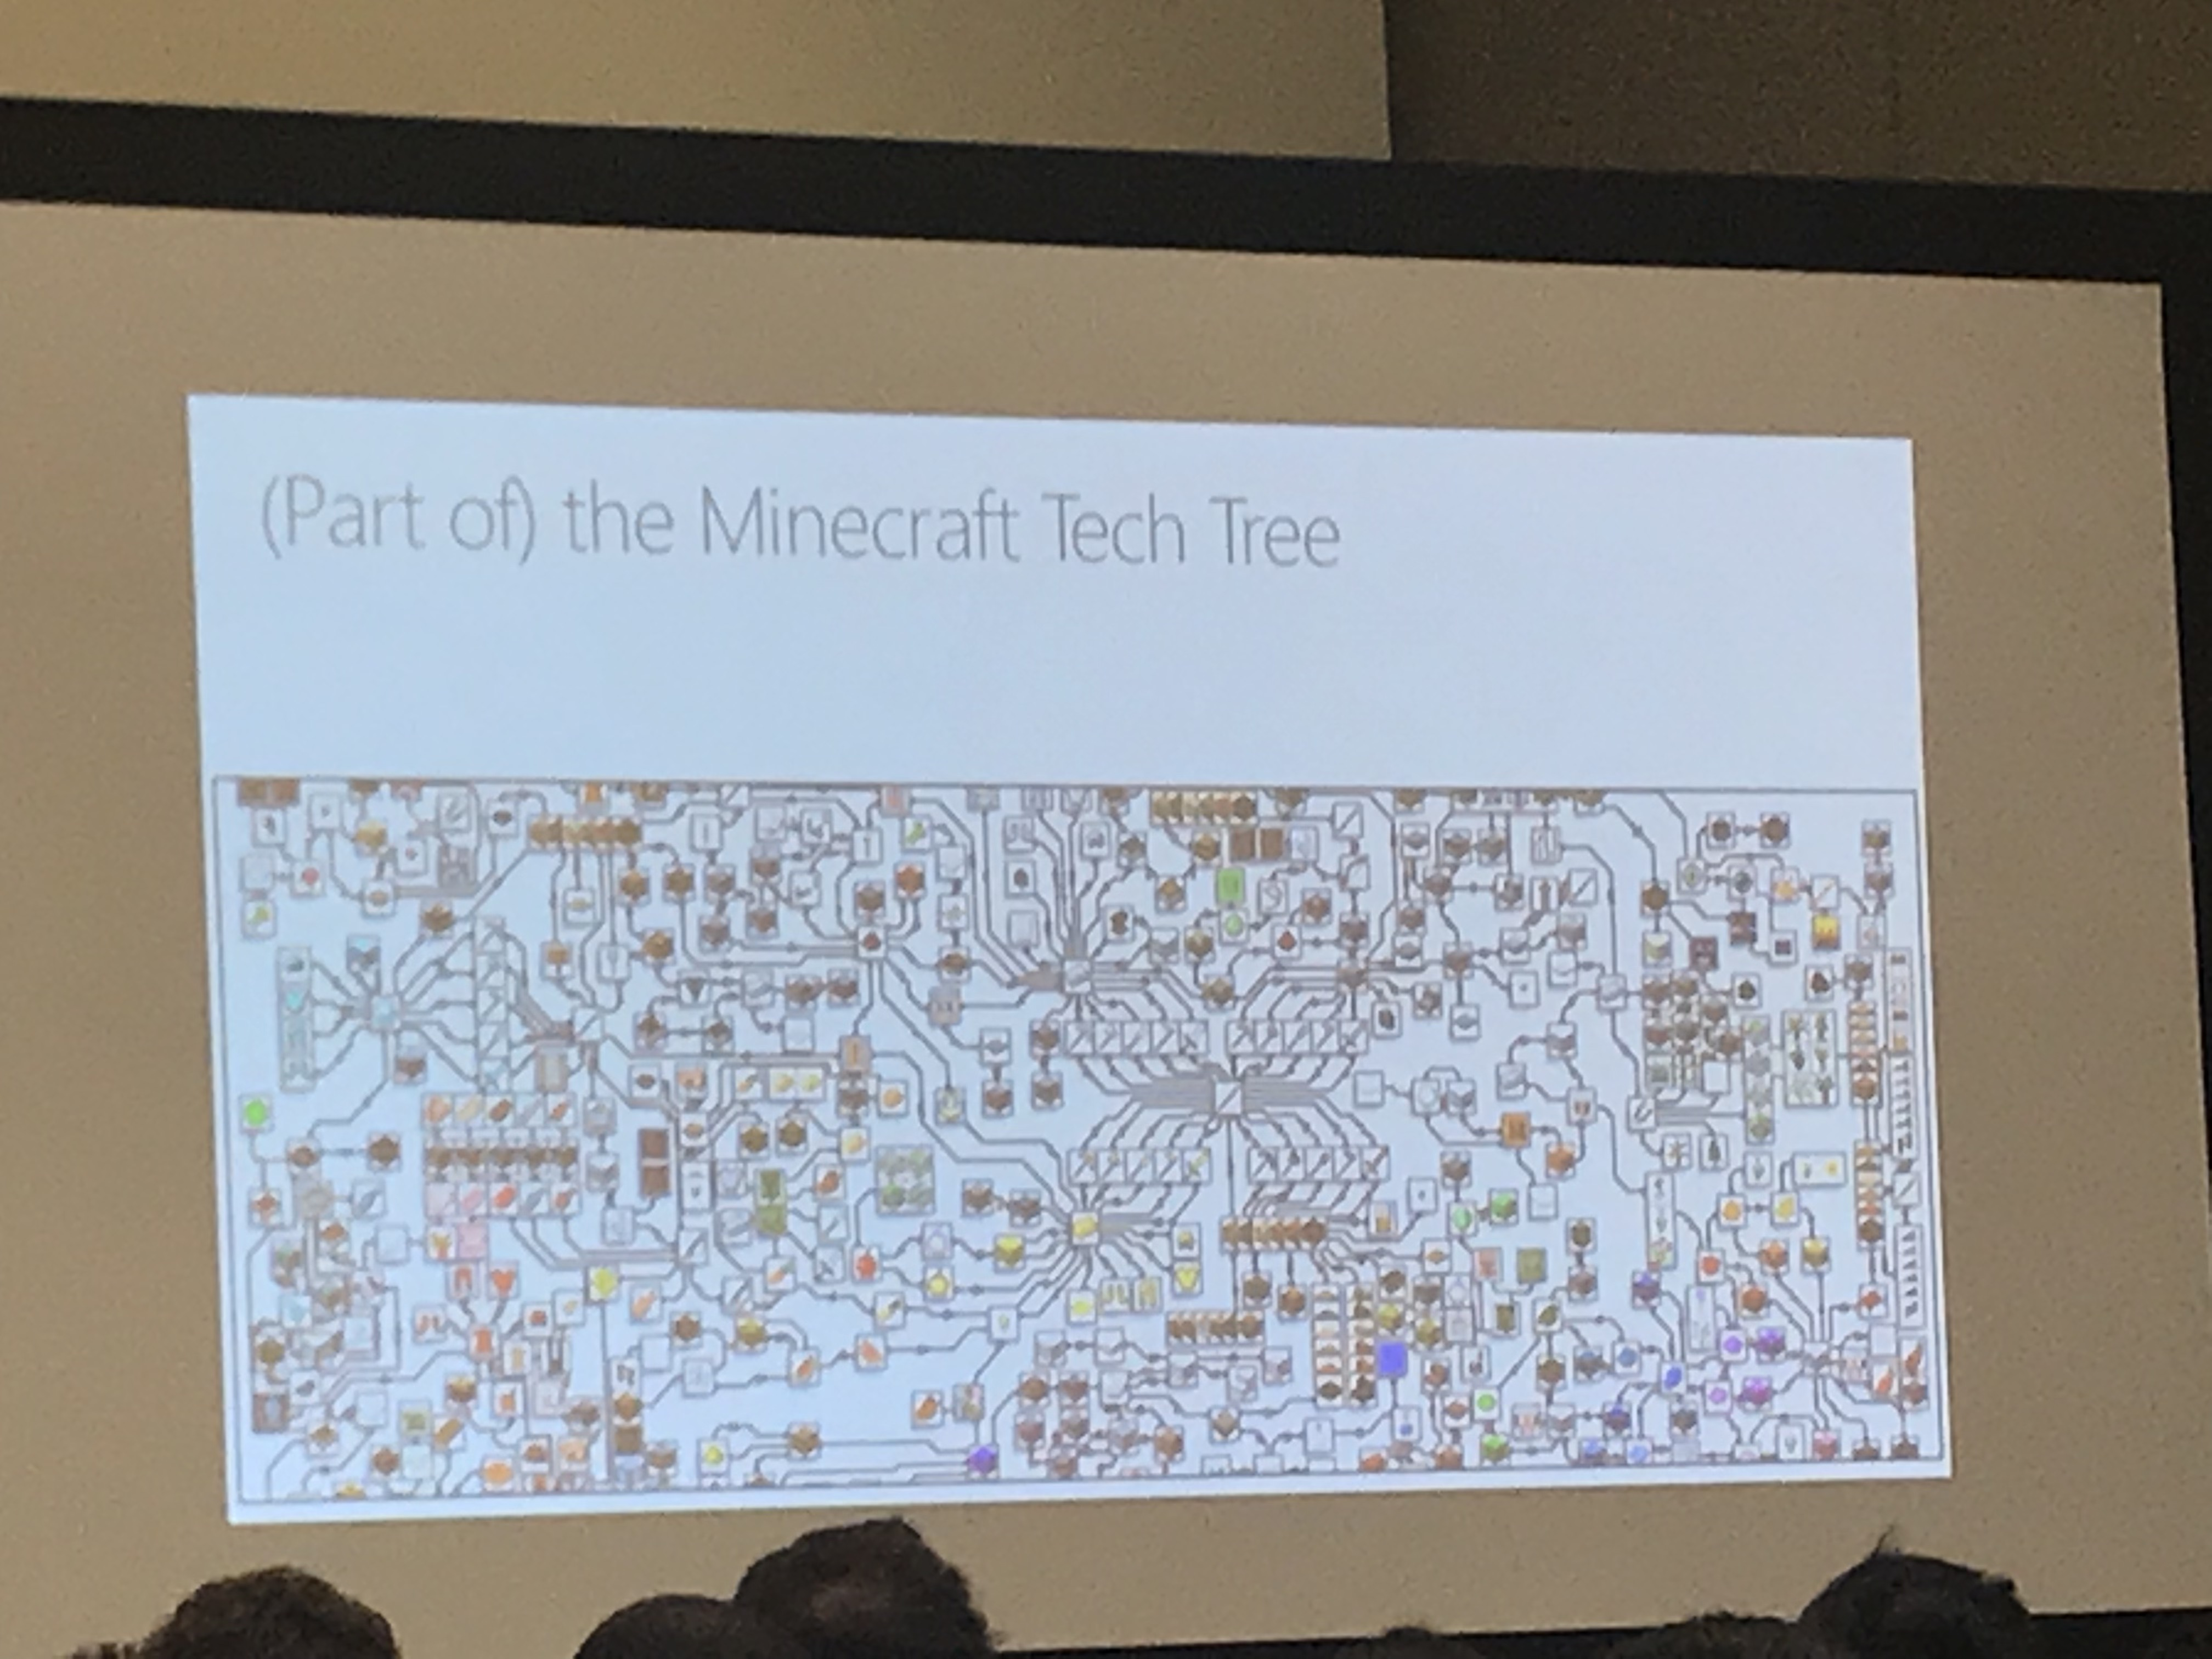
\includegraphics[width=0.4\textwidth]{images/mc_tree.JPG}
    \caption{Part of the tech tree in Minecraft}
    \label{fig:mc_tree}
\end{figure}

\subsubsection{Tejas Kulkarni on Object-Centric Representations RL}

{\bf Point:} The hard problems of RL:
\begin{enumerate}
    \item State estimation
    
    RL does not prescribe a detailed recipe to represent state. Hand specify or learn a state representation.
    
    \item Exploration
    
    And: how you explore depends on how you explore the world.
\end{enumerate}

This work: let's use self-supervised deep learning to learn object structure. \\

Example: an individual blind from birth can still draw rough object structure, including {\it perspective}~\cite{kennedy2006blind} -- see Figure~\ref{fig:drawing}. \\

\begin{figure}[h!]
    \centering
    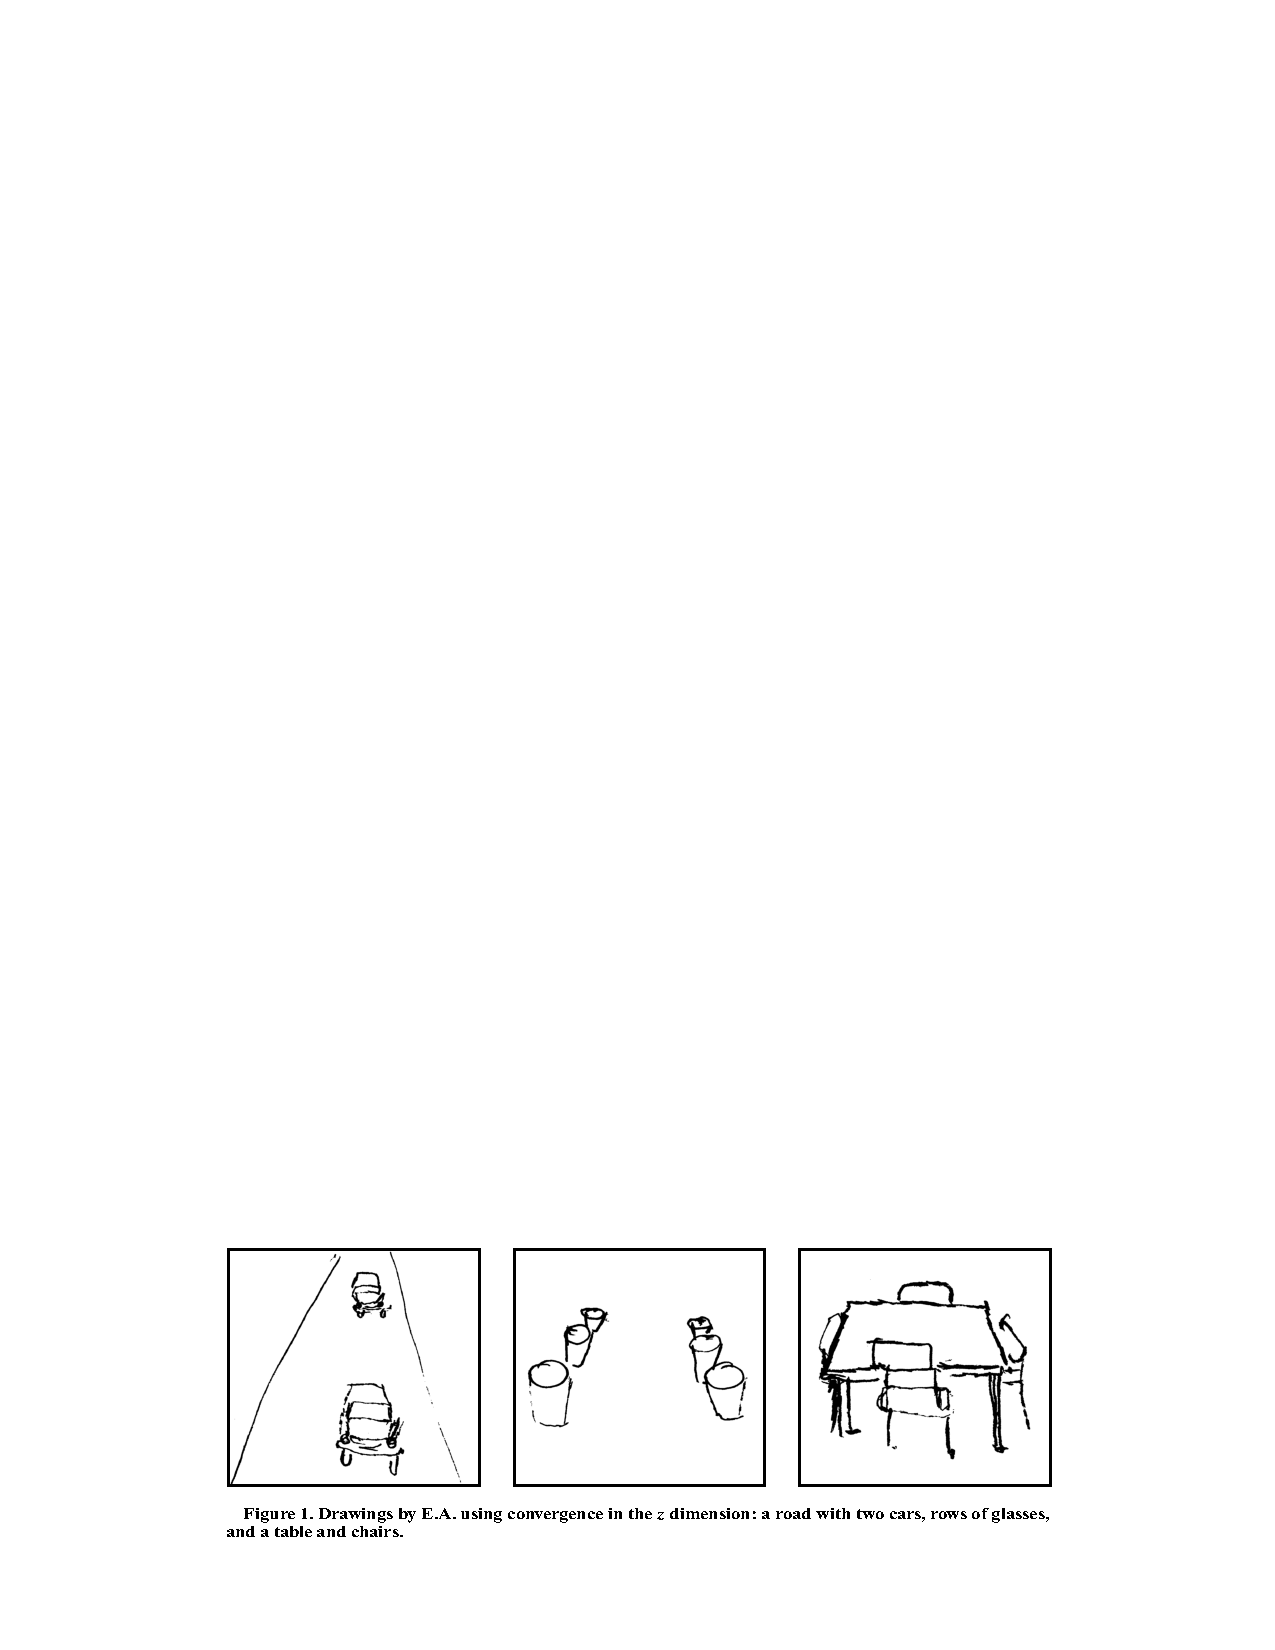
\includegraphics[width=0.5\textwidth]{images/drawing.pdf}
    \caption{Drawings from~\citet{kleinberg2016inherent}}
    \label{fig:drawing}
\end{figure}

Objects in particular are a fundamental and important abstraction.\\

Q: So, can we learn them?\\

Three properties from object-centric representation in physical domains:
\begin{enumerate}
    \item Capture spatio-temporal features at degrees of freedom.
    \item Long-term temporal consistency.
    \item Captures basic geometry of the environment.
\end{enumerate}

A: Yes! The ``Transporter" network (see Figure~\ref{fig:transporter}). %. \\

\begin{figure}[h!]
    \centering
    \subfloat[Transformer Network]{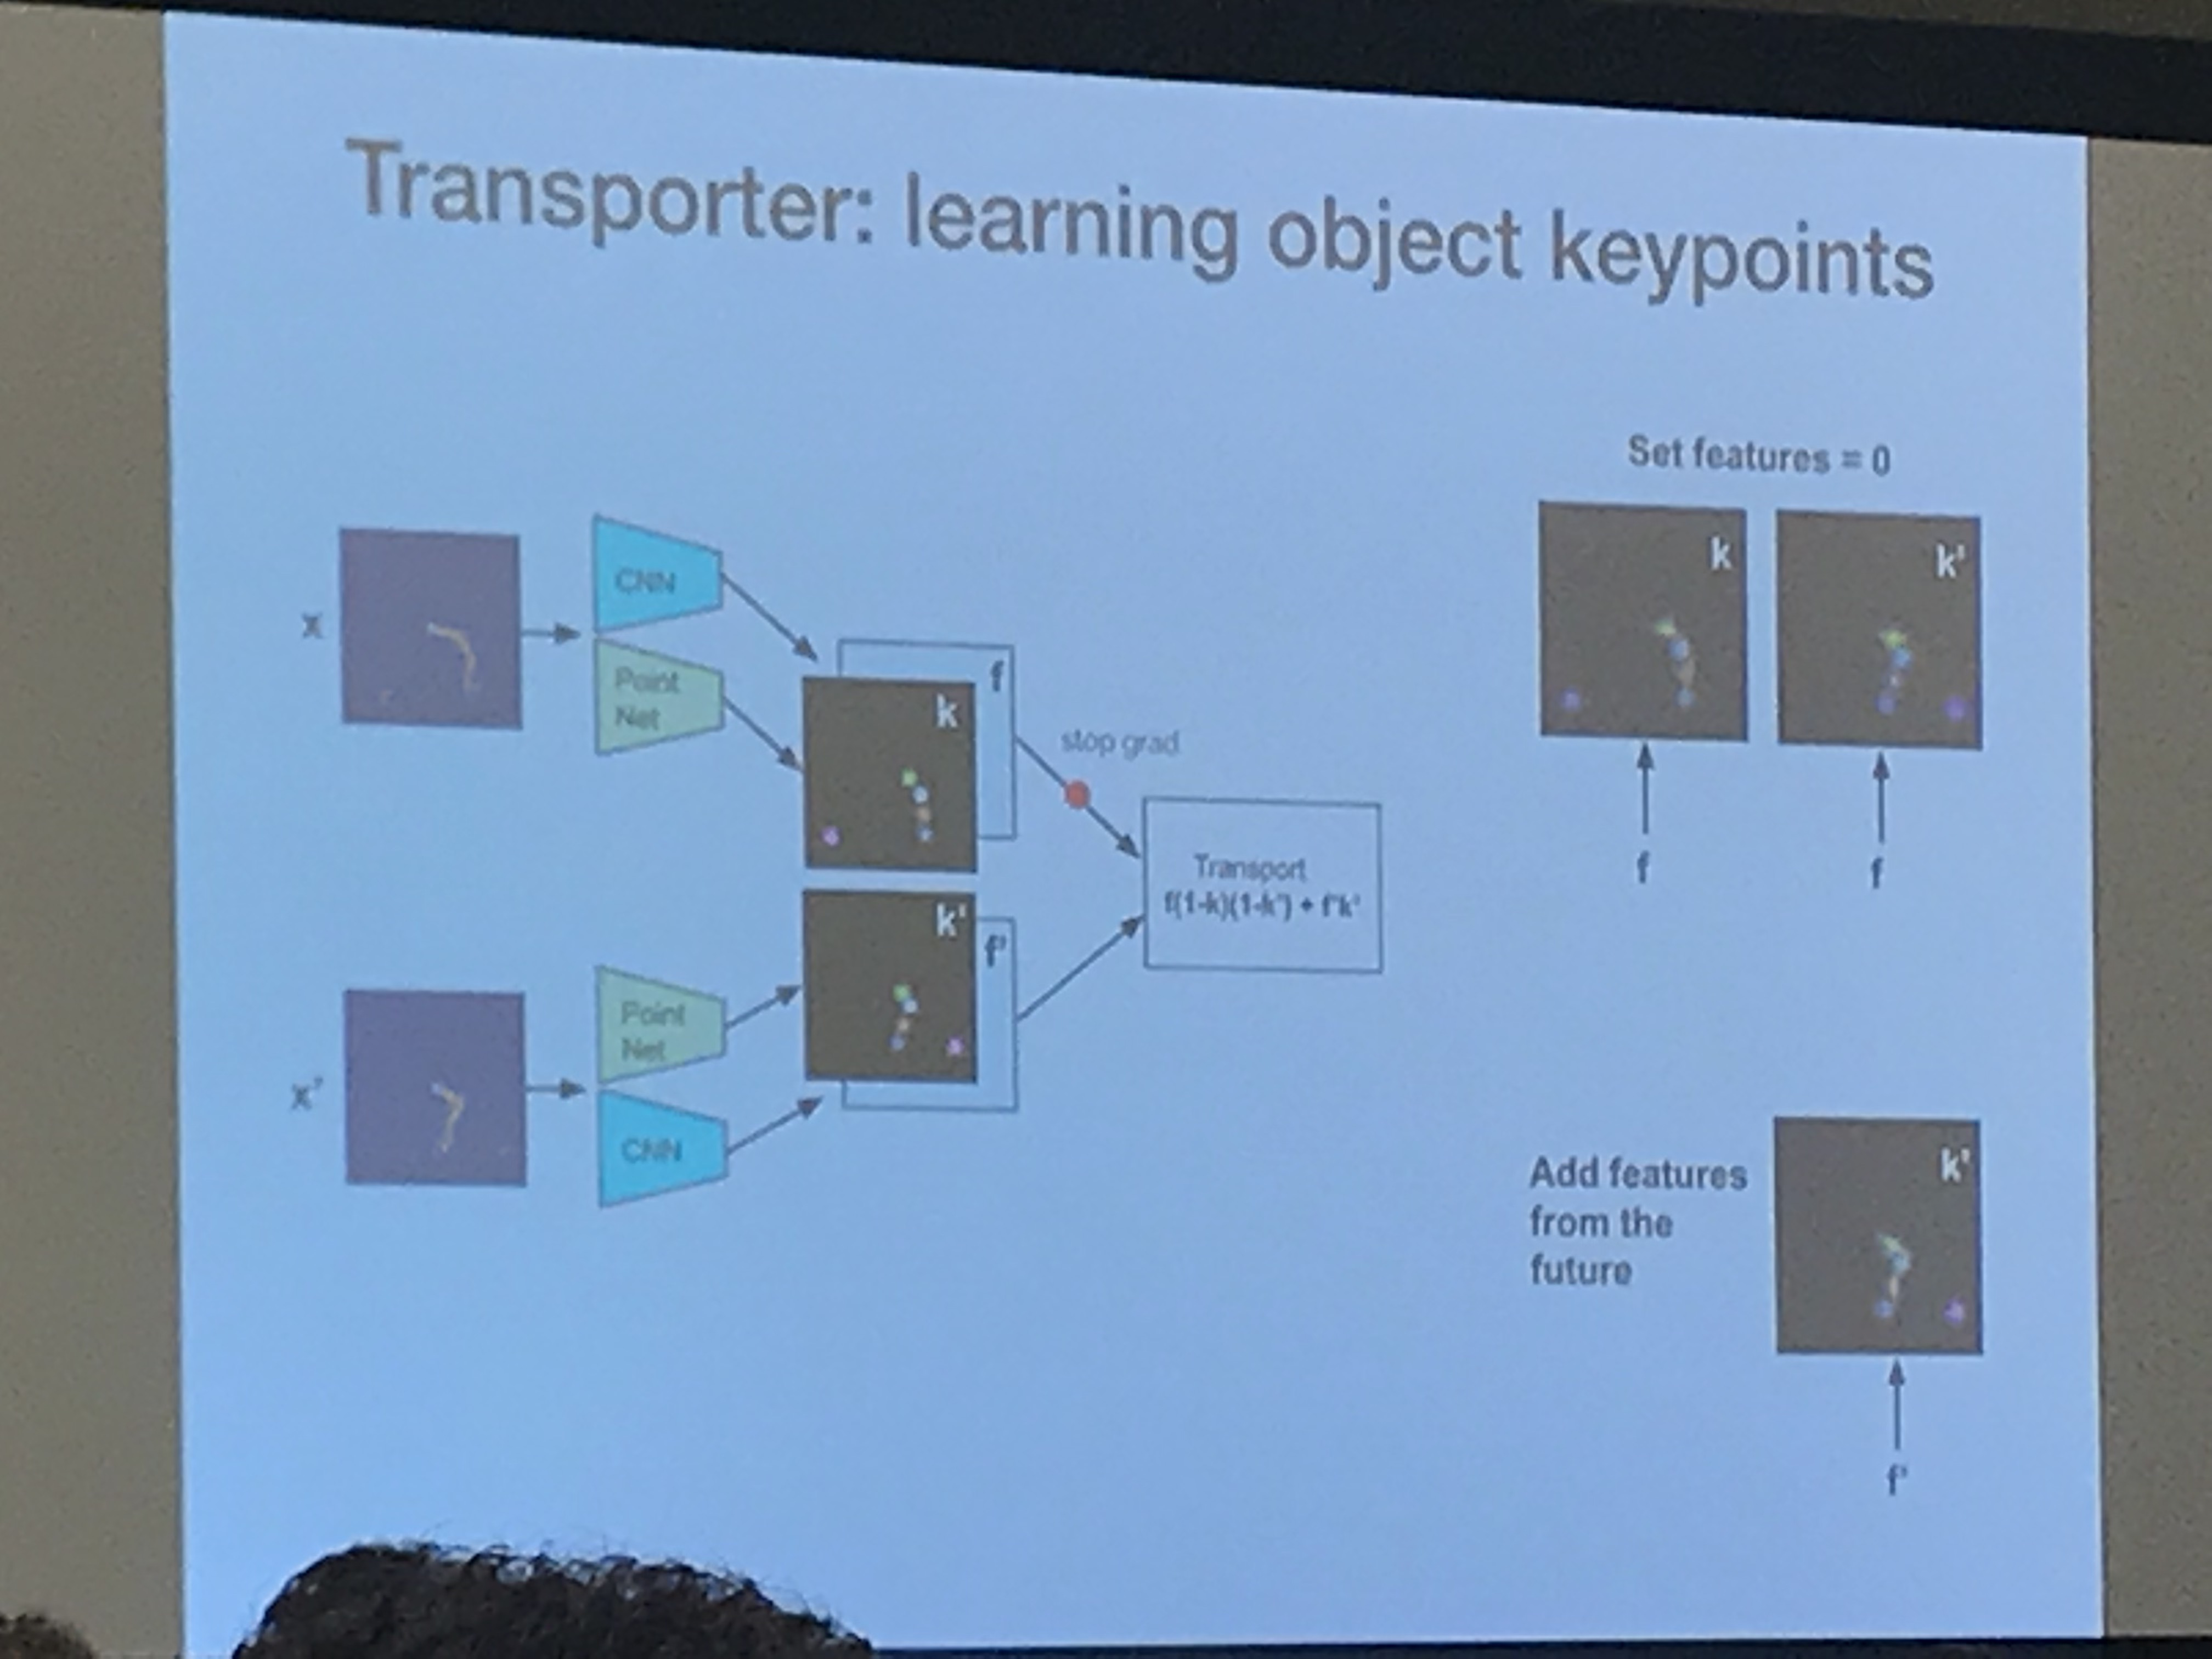
\includegraphics[width=0.4\textwidth]{images/transporter.JPG}} \hspace{5mm}
    \subfloat[Object Classification]{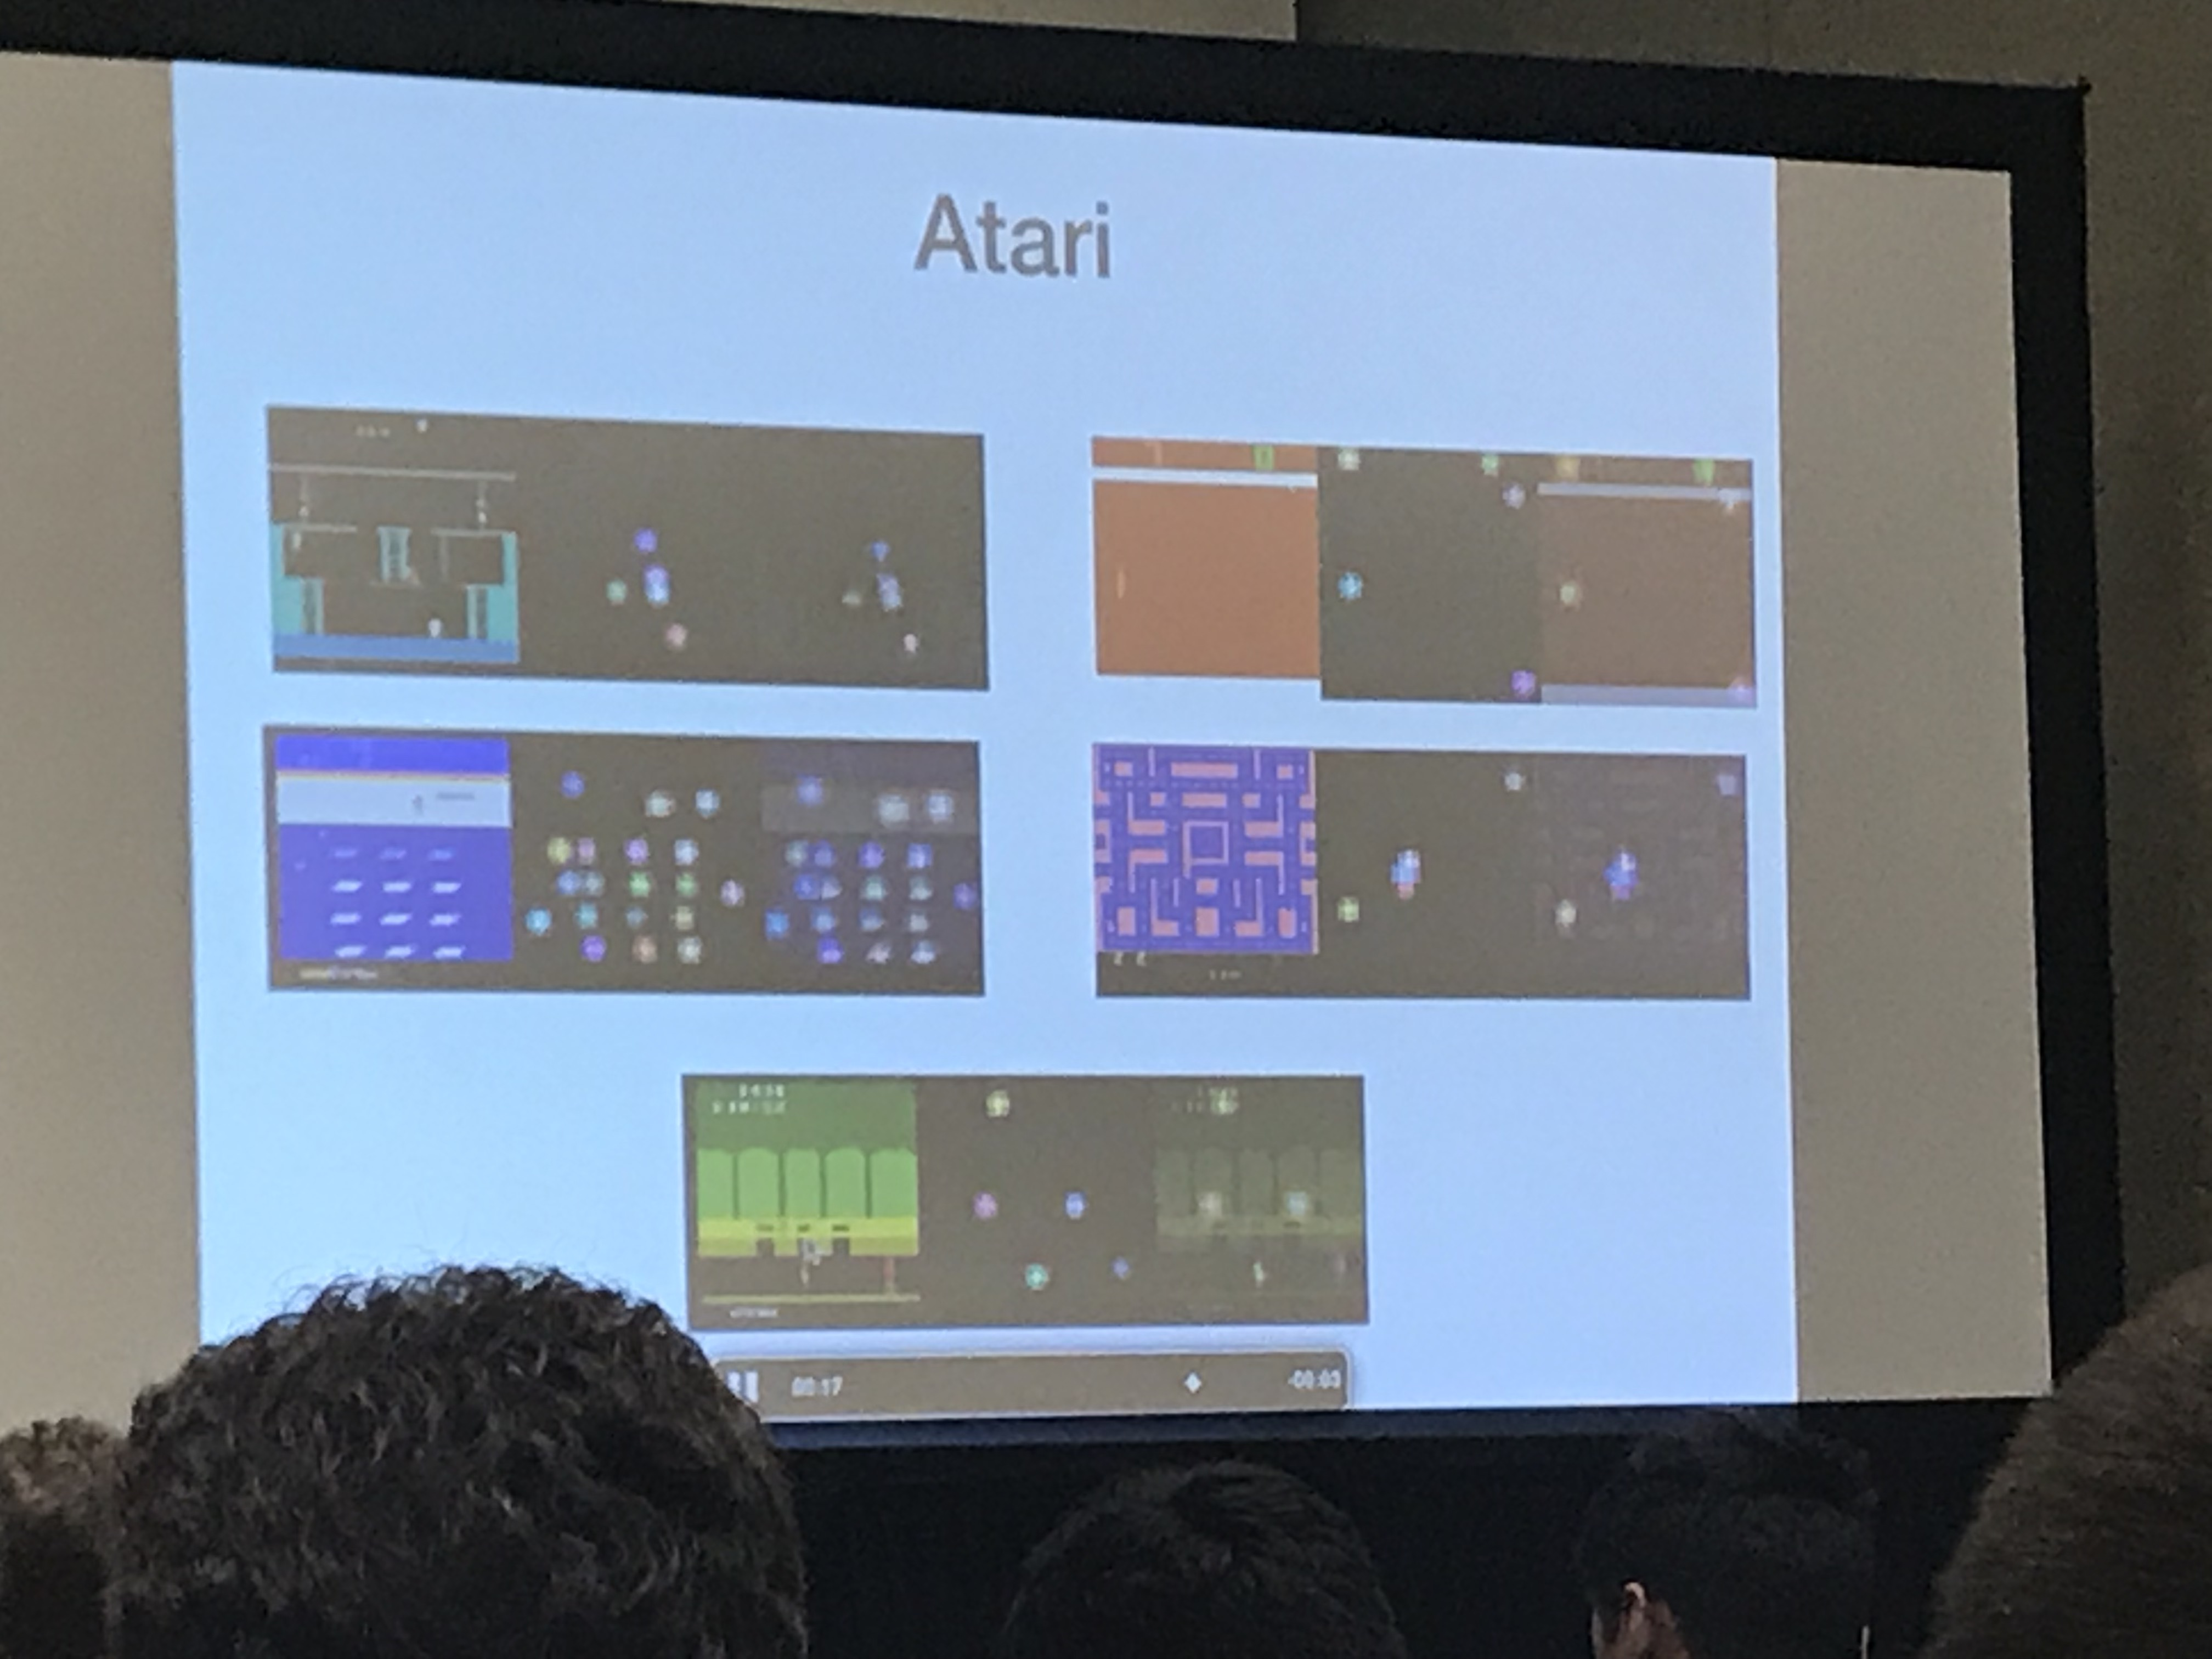
\includegraphics[width=0.4\textwidth]{images/objects.JPG}}
    \caption{Transporter Network (left) maps source to target image via compressed geometric representation, and some candidate objects found (right) in different Atari games.}
    \label{fig:transporter}
\end{figure}

$\ra$ Transporter network does a good job for capturing salient objects in image based problems like Montezuma. Trained on uniform random policy, and the result is a spatial map of where different objects area. \\

But: the above approach only tracks moving objects, not stationary ones. So, we can pair it with instance-based segmentation for finding stationary objects. \\

{\bf Next Stage:} Object-Centric RL and Planning in high dimensional domains, building on the earlier work by~\citet{diuk2008object}. \\

$\ra$ Key Problem 1: Structured exploration in the space of objects and relations. \\

$\ra$ Key Problem 2: Generalization in the form of self generated tasks in the space.

Object-centric HRL architectures~\cite{kulkarni2016hierarchical,dilokthanakul2019feature}. \\

Major frontier: data efficient RL in hard exploration settings like Montezuma. Idea: systematically explore in the space of objects and relations.

{\it Challenge Question:} In supervised learning, progress in representation learning and trasnfer learning for vision has been largely driven by ImageNet. NLP had its ``ImageNet" moment with GPT-2 and BERT. So, will there be a analogous ``ImageNet" moment in RL that allows us to learn general prupose data-driven priors? \\

A: Yeah, absolutely! I think we're almost there. Lots of folks working in this direction, I think we are right around the corner. 


\subsubsection{Tim Lillicrap on Learning Models for Representations and Planning}

Current State and Limitations of Deep RL:
\begin{enumerate}
    \item We can now solve virtually any single task/problem for which:
    \begin{enumerate}
        \item Formally specify and query the reward function
        \item Explore sufficiently and collect lots of data
    \end{enumerate}
    \item What remains challenging:
    \begin{itemize}
        \item Learning when a reward function is difficulty to specify
        \item Data efficiency and mult-task transfer learning
    \end{itemize}
\end{enumerate}

We measure outcomes via: $R(\tau) = \sum_{t=0}^T \gamma^t r_t$, with the objective function:
\begin{equation}
    J(\theta) = \int_\mathbb{T} p_\theta(\tau) R(\tau) d\tau.
\end{equation}

But: In model-free RL we tend to throw away what we know about the task to solve it. \\

Clear structure to introduce: plan with a model. \\

$\ra$ Tricky! Getting this model is really hard. If we can get it, we know it can be really powerful (see AlphaZero~\cite{silver2018general}). \\

{\bf Problem:} Planning with learned models is really hard. (Tim said it became a running joke to started up a model-based RL project at DeepMind in the last few years: no one expected it to work). \\

Idea: Hybrid model-free and model-based approaches. By augmenting previous algorithms with a learned model did in fact help on a goal-finding task. \\

Planning with Learned Models: PETS~\cite{chua2018deep}, Deep Planning Network (Planet)~\cite{hafner2018learning}. \\

Experiments: continuous control from image observations (finger, cheetah, cup, etc). \\

$\ra$ Some versions of this end up working well! Around 1k-2k episodes it can solve image-based mujoco problems. \\

{\bf Conclusions:}
\begin{itemize}
    \item Model-based algorithms hold promise of addressing data efficiency and transfer learning limitations.
    \item Beginning to develop working recipes that allow planning with models in unknown environments.
    \item Necessary and sufficient conditions for planning with learned models are unclear.
    \item Much work remains!
\end{itemize}


{\it Challenge Question:} What are the trade-offs in rolling value estimation and perception into the same architecture? \\

Tim A: I don't know anyone that's systematically studied this kind of thing, but it's definitely important to study it more. Some insights can be gathered from AlphaZero, ELO rating analysis. Lots more to do! 

\subsubsection{Karthik Narasimhan on Task-agnostic Priors for RL}

Current State of RL: success of model-free RL approaches (see: Go, DOTA). \\

$\ra$ All of these feats require huge amounts of time and samples (like 45,000 years of gameplay for DOTA). \\

$\ra$ Little to no transfer of knowledge. \\

Recent Approaches:
\begin{itemize}
    \item Multi-task policy learning
    \item Meta-learning
    \item Bayesian RL
    \item Successor Representations
\end{itemize}

Observation: all approaches tend to learn policies, which are rigid and hard to transfer to other tasks. \\

Solution: model-based RL.\\

$\ra$ Approach: bootstrap model learning with task agnostic priors. The model is 1) more transferrable, 2) expensive to learn but can be made easier with priors. \\

Q: Can there be a universal set of priors for RL? \\

A: Look to how humans learn new tasks. These priors seem to come from 1) a notion of intuitive physics and 2) language. \\

{\bf Project 1:} Can we learn physics in a task agnostic way? Moreover, can this physics prior help sample efficiency of RL? \\

Lots of prior work in this area, but they are task-specific. \\

$\ra$ This work: learn physics prior from task-independent data, decouple the model and policy. \\


Overview of approach:
\begin{itemize}
    \item Pre-train a frame predictor on physics videos
    \item Initialize dynamics models and use it to learn policy that makes use of future state predictions.
    \item Simultaneously fine-tune dynamics model on target environments.
\end{itemize}
Two Key Operations: 1) isolation of dynamics of each entity in the world, 2) accurate modeling of local spaces around each entity. \\

Experiments: PhysWorld and Atari -- in both cases, use videos containing demonstrations of the physics of the environment to do some pre-training of the dynamics model (in Atari, pre-training is still done in PhysWorld). Results show the approach works very well, both at 10-step prediction and at helping sample efficiency in RL. \\


{\bf Project 2:} Can we use language as a bridge to connect information we have about one domain to another, new domain? \\

Overview of approach:
\begin{itemize}
    \item Treat tanguage as task-invariant and accessible medium.
    \item Goal: transfer a model of the environment using text descriptions.
    
    Example: ``Scorpoins can chase you". Might be able to learn a model that places high probability on the scorpoin moving closer to tthe agent location.
    
    \item Main technique: transfer knowledge acquired from language to inform a prior on the dynamics model in a new environment.
\end{itemize}


Conclusions:
\begin{enumerate}
    \item Model-based RL is sample efficient but learning a model is expensive
    \item Task agnostic priors over models provide a solution for both sample efficiency and generalization
    \item Two common priors applicable to a variety of tasks: classical mechanics and language.
\end{enumerate}


{\it Challenge Question:} Lots of success in Deep RL. New push into hybrid approaches like cross-domain reasoning, using knowledge from different tasks to aid learning, and so on. What are the greatest obstacles on the path to mid-level intelligence? \\

Karthik A: I would emphasize the need for distributional robustness and transfer -- need to look at agents that can transfer across similar domains. Some obstacles involve 


\subsubsection{Ben E., Lisa L., Jacob T. on Priors for Exploration and Robustness}

Challenges in RL today:
\begin{enumerate}
    \item Exploration
    \item Reward function design
    \item Generalization
    \item Safety
\end{enumerate}

$\ra$ Priors are a powerful tool for handling these challenges. \\

Q: Can we learn useful priors? \\

A: Yes! This work is about a general algorithm for learning priors. Idea is to frame RL as a two player game, with one player being an adversary choosing a reward function. \\

{\bf Project 1:} State marginal matching.\\
$\ra$ Idea is to try to maximize policy state distribution to some objective distribution. Minimize $KL$ between $\pi^*$ and $\pi$. \\

Experiments: test for exploration and meta-learning capacity of the algorithm. Tested with locomotion and manipulation tasks. Their approach works quite well. \\

{\bf Project 2:} Priors for Robust Adaptation. \\

$\ra$ RL with unknown rewards: assume we're given a distribution over reward functions. Then, sample a new reward function and optimize with respect to it. \\

Main approach: compute the Bayes-optimal policy, and then perform regular RL.



\subsubsection{Doina Precup on Temporal Abstraction}

Guiding Q: How can we inject temporal abstraction into options? \\

$\ra$ Where do options come from? Often, from people (as in robots). \\

$\ra$ But what constitutes a good set of options? This is a {\it representation} discovery problem. \\

Earlier approach: options should be good at optimizing returns, as in the Option-Critic~\cite{bacon2017option}. Option-critic learns option representations that yield fast in-task learning but also effective transfer across tasks. \\

{\bf Point:} Length collapse occurs -- options ``dissolve" into primitive actions over time. \\

{\bf Assumption:} executing a policy is cheap, deciding what to do is expensive. So, can use options with an explicit {\it deliberation cost} in mind~\cite{harb2018waiting}. \\

That is, can define a new value function based on the deliberation cost:
\[
Q(s, o) = c(s,o) + \sum_{s'} P(s' \mid s,o) \sum_{o'} \mu(o' \mid s') Q(s',o'),
\]
with $c(s,o)$ some cost of deliberation. \\


Experiments: on Atari, with and without deliberation cost (as a regularizer). Indeed find that options take longer before terminating (which was the intended goal). \\

 Q: Should all option components optimize the same thing? (Should $\mc{I}, \beta, \pi$ all be geared toward maximizing rewards?) \\
 
 A: Based on the deliberation cost work, one might think that aspects of the option should take these regularizers into account. See, for instance, the recent work by~\citet{harutyunyan2018learning}, or the termination critic~\cite{harutyunyan2019termination}.\\
 
 {\bf Idea:} Bottleneck states -- we might want options that take us to these bottlenecks. \\
 
 $\ra$ Drawback: expensive both in terms of sample size and computation. \\
 
Discussion:
\begin{itemize}
    \item Priors can be built into option construction via optimization criteria
    \item Termination and internal policies of options could accomplish different goals
    \item {\it **Biggest Open Question:} how should we empirically evaluate lifelong learning AI systems?
\end{itemize}

How do we assess the capability of a lifelong agent?
\begin{enumerate}
    \item No longer a single task!
    \item Returbns are imporant but too simple
    \item How well is the agent preserving and enhancing its knowledge?
\end{enumerate}

$\ra$ Proposal: hypothesis-driven evaluation of continual systems. That is, take inspiration from other fields (psychological, for instance).


{\it Challenge Question:} Lots of recent work applies deep RL to existing algorithms in HRL and option discovery. What has deep RL brought to the table? Do they fix all of the problems or do we need some new paradigm shift? \\

Doina A: Neural nets brought to HRL roughly what they brought to regular RL -- aspects of the feature discovery problems have effectively been solved. On one hand that's great, because we have a solution. On the other hand, we are still lacking in methods that truly do knowledge discovery. Deep nets are not really an answer to that process. There's a temptation to take a deep net throw it at a problem and put some HRL objectives on the top. Yes, that might work, but it doesn't lead to decomposable or modular knowledge. We've mode lots of progress but perhaps it is a good time for us to take a step back and do fancier things in terms of state abstraction and options. 

\subsubsection{Jane Wang on Learning of Structured, Causal Priors}

{\bf Point:} Structured priors enable faster learning. \\

$\ra$ {\it Causal} priors in particular can enable faster learning (by improving exploration, generalization, credit assignment, and so on). \\

Causal reasoning is a rich field, so, some background:
\ddef{Bayes Net}{A probabilistic graphical model that represents a set of variables and their conditional probability distribution in the form of a directed acyclic graph (DAG)}

\ddef{Causal Bayes Net}{Bayes net where arrows represent causal semantics}

\ddef{Intervention}{Fixing a value of a variable, disconnecting it from its parents.}

\ddef{Do-calculus}{A set of tools for making causal inferences given observational data}

Can ask three levels of questions:
\begin{enumerate}
    \item Association: are drinking wine and me having a headache related?
    \item Intervention: If I go drink wine, will I have a headache?
    \item Counterfactuals: go back in time and ask, what if I had drank wine? Would I have a headache?
\end{enumerate}

\begin{figure}[h!]
    \centering
    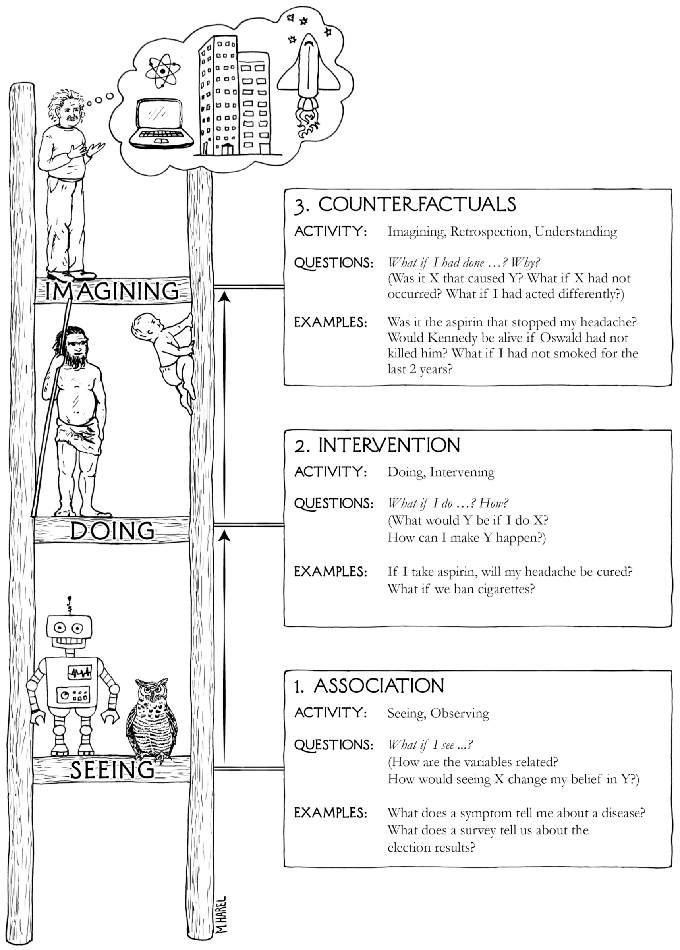
\includegraphics[width=0.3\textwidth]{images/ladder.png}
    \caption{Pearl's ladder of causality}
    \label{fig:ladder_of_caus}
\end{figure}

Q: How does causal reasoning manifest in humans? \\

A (babies): Babies less than a year old do not demonstrate causal knowledge, but do have a sense of physical continuity. \\

A (2 year olds): Can learn predictive relationships between events, but can't sponetaneously make interventions based on causal understanding. \\

A (3-4 year olds): Can infer causal maps from observing conditional dependencies. \\

A (4-5 year olds): Can make informative targeted interventions based on causal knowledge. \\

A (adolescence): Strategies for causal learning continue to improve. \\

A (adults): Evidence of an associative bias, a ``rich-get-richer" prnciple: one variable is more likely to be present if others in the causal model are also present. \\

{\bf Overall:} evidence suggests that children display ability to perform causal inference from observation (roughly consistent with Bayesian inference). More sophisticated forms of reasoning (performing novel informative interventions) come online later as a result of experience. \\

But: major deviations from rationality/good inference. \\

$\ra$ Reasons for deviations:
\begin{enumerate}
    \item Formal models of causal reasoning optimize difference cost functions.
    \item Humans do not optimize for a specific causal graph, but a flexible one.
    \item 
\end{enumerate}

{\it Takeaway:} A structured universe of tasks $\implies$ we should use structured priors. \\

{\bf Idea:} Meta Learning of causally inspired priors. Similarly to previous talks, assume a distribution of tasks, want to learn some priors that lead to sample efficient learning in new tasks. \\

Experiments: 1) learning from observations on causal networks (can the agent learn some causal structure from a DAG?); 2) learning from interventions; 3) Learning from instance specific info. \\

{\it Challenge Question:} Why does deep Rl seem to struggle with out-of-sample generalization compared to other domains? ?

Jane A: In RL, lots of ways to be out of sample (in contrast to supervised learning), so it's much harder. Generalization is just harder because lots of things can change: state, action, policy, transition function, reward, function, and so on. RL also requires an ongoing interaction with the environment -- input is really dependent on policy, so input will change as you update policy.

\subsubsection{Panel: Matt, Jane, Doina, Sergey, Karthik, Tejas, Tim}
\label{sec:panel}
Q: What is the role of structure vs. data? \\

Tim: Question is loaded. Depends on what you want to do: if you want to get good at a niche, specify more. If you want a general learning algorithm: specify less. \\

Tejas: Yes! The article talks about search, but to me the big question is making domains ``computable" (simulatable). The article is misguided: where do the primitives come from? Can't rely on the data to give you primitives. We should radically add structure. There are certain truths we can and should exploit to search effectively (objects, agents, physics). \\

Karthik: Humans have evolved many things over time that are key to our intelligence. Definitely having the right kind of inductive biases and structured priors to get things to work.  \\

Matt: I want to push back on that, because I hear it from psychologists. The assertion is often made that because babies have strong inductive biases, our agents have inductive biases. But its not obviously a constraint we need to fight in designing agents. I don't buy the argument that babies tell us that much. I love Rich Sutton but I think we have to start with structure (like CNNs). Also potentially a formal consideration; the abstractions we need to learn will require an arbitrarily small. \\

Doina: There's one thing to say we need only data, and there's another thing to say that we always have to learn from scratch. Right now we don't incorporate the right kind of structures so that we don't have to learn from scratch. We use some ideas (CNNs, gradient descent), but we want to avoid adding too much structure, too. \\

Jane: One thing in Rich's essay (which I agree with about 80\%) is that he said our brains/the environment are irredeemably complex. I don't agree with that. Neuroscience and cognitive science have been making great strides in understanding our brains. \\

Sergey: This question is different because of a methodological issue. ML is a mathematical/philosophical/scientific field. So, we're good at some things, but not at all. We've been great at making computer vision systems, language systems, and so on. In RL we've mostly been focused on solving some problems but that's been a proxy to a much grander vision that we hope to work. That's where the methodological flaw catches us. It's very easy to get improvement from bias in small problems. \\

Doina: I think that's true in the rest of ML too (Sergey: I didn't want to offend everyone! \dnote{tongue in cheek :)})). In NLP, yes, we can do some tasks but can't really do all tasks. In all of ML, we make tasks that are examples that help us improve algorithms/models, but ultimately we need to go to a more complex setting. \\

Matt: At the risk of engaging too much in the philosophical side of ML. We don't want to build in inductive biases that are too concentrated on one domain. In ML, we do tend to have a sense of the general domain we anticipate our agents being deployed in. We just have to make our choices about what ontology you want to buy into.\\

\spacerule

Q: We don't really know what tasks to train on in RL, especially in lifelong RL/multitask RL/meta RL. Any thoughts on defining the problem in a more precise way? \\

Doina: Simulation is obviously necessary. Think about human learning: babies have parents, who have an important role. How to build interesting and rich simulations that can be used for complex RL evaluation tasks? Well, one thing we can do is look more seriously at multi-modal data. \\

Sergey: Important to think about what RL would look like as a data driven field instead of a simulation driven field. If we don't we might be stuck in a regime where we don't think much about generalization and other core problems. We could think about RL tasks as being started with {\it data}, which is closer to the kinds of RL algorithms we might want that live in the real world. Kind of crazy to imagine an algorithm could learn a complex task {\it tabula rasa}.\\

Tejas: I agree with everything that was said. Generalization only matters when your data is limited. One way to think about that is when agents can generate their own tasks. We should think of metrics and measurements which incentivize researchers and platforms where agent can create lots of tasks, play in those tasks to learn more complex behaviors. \\

Tim: Question for Sergey: approaching RL in a data driven mode, how much of that needs to be done with real world data vs. simulation? \\

Sergey: I'll answer that with a question: what if we wanted to make a better image classifier? We do it with real data in vision because it's easier to make progress. So, in RL, it's easier too, because of the inherent complexity/diversity in the real data. \\

Doina: Bit of a different problem b/c we need trajectories. Lots of trajectories. Trajectories generated by people might be very different too. Might be really hard to understand/learn from whole trajectories. \\

Sergey: Might not be that hard. Can collect lots of self driving car data, grasping data, and so on, relatively easily. \\

Jane: Tend to agree with you (Sergey). One question about real data: can we make guarantees about moving beyond that labratory data? \\

Sergey: That's where you need to be really careful. \\

Tejas: from first principles, no reason we can't make a simulator that's indistinguishable in terms of graphics and physics. Just a matter of time before we have a simulator that can replace real world data. \\

Sergey: Sure! But might be really slow. Why wait? \\

\spacerule

Q: What's the main reason to used model-based vs. model-free learning? \\

Karthik: Learning a model of the world can give you far more flexibility about what you can accomplish. In model free learning, you tend to just have on policy/value function, it wont generalize well/transfer across tasks. Can cover roughly 90\% of things that can happen with a (good) model. \\

Doina: Not so sure the distinction is salient. Models can be thought of as generalized value functions, where things become much more blurry. Might end up with model-based RL that is much less efficient because learning the mapping from obserbation to observation is very hard. To do this, need to understand the effects of your actions vs. understand what other variables are important for policy/value function. This latter component might be much simpler than the former. Might need to rethink the nature of our models. We should build models that are small bricks. \\

Matt: That resonates! Fascinated by grey the distinction is between model-free and model-based. For a number of years in neuroscience this distinction was treated as very categorical. But, we've realized it's much messier. We're focused on models that can maximize value, but the situation changes when we instead focus on agents that can transmit knowledge to other agents via teaching or communication. We likely need very different models for these kinds of tasks. \\

Sergey: I think the two approaches are the same. They're similar, at least. RL is about making predictions (usually), but it's important to realize there's a lot of knowledge contained in some of the things agents predict like the value function (\dnote{very clever dollar bill example Sergey used: imagine you wanted to predict the number of dollar bills in front of you, and maximize this value. To do this you basically need to model everything in the world.})

Tejas: Lots of domains that have nothing to do with rewards or reward maximization, like coming up with number theory or computability. \\

Sergey: It's not the only way to develop knowledge about the world. But if there's something that has a meaningful effect on your environment, then you'll need to predict them in order to estimate/maximize your value function. \\

Jane: One thing about learning these models just from interaction -- in the real world, things are not necessarily disentangled in the way you might like. \dnote{I missed the rest :(} \\

\spacerule

Q: Is there a general recipe for extracting understanding from human intelligence for RL? \\

Matt: Meta learning (mic drop). Look at the history of AI: AI winter was partially caused by the failure of trying to encode all knowledge into our agents. We definitely want to avoid that with inserting the right structures.\\

Tejas: Good inductive biases are ones that will never go away. Desiderata for those are that they are truths. How do we find truths? A few scientific ways to do that: notions of agency are true, objects are true. Put these kinds of truths into the agents' head, I think we'll have agents that do the right thing. \\

Q: Is anything really ``True"? \\

Tejas: Yes, otherwise it's just soup. There's no existence without it. An agent is an object with goals, and objects are true. We can try to learn these invariant truths. \\

Doina: With the risk of circling back: one of the lessons that we have been learning over and over again is that putting too much stuff into the agent's head can be detrimental. See: AlphaGo. Put in a bit of knowledge, let it find its own knowledge from its own data. Lots of the structure we have in deep RL are useful, but some are probably not useful. \\

Tejas: if you don't assume anything then what? Can we assume a model of an agent? \\

Sergey: Lots of things that are true and obvious. It's okay to learn that from data. Naybe it's better, because then it knows how to learn those true things to other ones. Better for my students to figure some things on their own, for instance. \\

Tim: Tend on the side of fewer inductive biases, and we'll tend to keep coming back to that. As we get more data, it might be easy to discovery the essential inductive biases from the data we have around. Humans/animals genetic code don't contain that many bits that are sitting in our DNA that produces our brains/bodies. Rediscovering those inductive biases might not be that hard, so we should tend to only lightly add inductive biases. \\

\spacerule

\dnote{Running out of battery: missed the last question!}